\documentclass{ieeeaccess}
\usepackage{cite}
\usepackage{amsmath,amssymb,amsfonts}
\usepackage{algorithmic}
\usepackage{graphicx}
\usepackage{textcomp}
\usepackage{booktabs}

\usepackage{bm}
\makeatletter
\AtBeginDocument{\DeclareMathVersion{bold}
\SetSymbolFont{operators}{bold}{T1}{times}{b}{n}
\SetSymbolFont{NewLetters}{bold}{T1}{times}{b}{it}
\SetMathAlphabet{\mathrm}{bold}{T1}{times}{b}{n}
\SetMathAlphabet{\mathit}{bold}{T1}{times}{b}{it}
\SetMathAlphabet{\mathbf}{bold}{T1}{times}{b}{n}
\SetMathAlphabet{\mathtt}{bold}{OT1}{pcr}{b}{n}
\SetSymbolFont{symbols}{bold}{OMS}{cmsy}{b}{n}
\renewcommand\boldmath{\@nomath\boldmath\mathversion{bold}}}
\makeatother

\def\BibTeX{{\rm B\kern-.05em{\sc i\kern-.025em b}\kern-.08em
    T\kern-.1667em\lower.7ex\hbox{E}\kern-.125emX}}

\graphicspath{{paper/figures/}{figures/}{./}}
% Auto-generated numeric macros from src/analyze.py (\R... commands).
\newcommand{\RnComp}{66}
\newcommand{\RnCompCand}{68}
\newcommand{\RnCompTotal}{69}
\newcommand{\RnCourses}{442}
\newcommand{\RnLinks}{1002}
\newcommand{\RovMultiBig}{3.18}
\newcommand{\RnLargePool}{50}
\newcommand{\RovRetrBig}{3.40}
\newcommand{\RdiffRetr}{0.20}
\newcommand{\RpRetr}{0.00932}
\newcommand{\RnHallComp}{5}
\newcommand{\RnSelNaive}{15.0}
\newcommand{\RnSelRetr}{4.6}
\newcommand{\RnSelMulti}{7.7}
\newcommand{\RrelRetr}{3.62}
\newcommand{\RcovRetr}{3.21}
\newcommand{\RcovMulti}{3.02}
\newcommand{\RjudgeCost}{2.15}
\newcommand{\RgenCostTotal}{0.10}
\newcommand{\RmedCand}{11}
\newcommand{\RmaxCand}{106}
\newcommand{\RovNaive}{2.88}
\newcommand{\RovRetr}{3.21}
\newcommand{\RovSingle}{3.05}
\newcommand{\RovMulti}{3.02}
\newcommand{\RrelMulti}{3.65}
\newcommand{\RordMulti}{2.70}
\newcommand{\RordNaive}{2.27}
\newcommand{\RordSingle}{2.62}
\newcommand{\RordRetr}{2.67}
\newcommand{\RcovNaive}{2.88}
\newcommand{\RminNaive}{95}
\newcommand{\RminSingle}{95}
\newcommand{\RminMulti}{100}
\newcommand{\RhallMulti}{3.1}
\newcommand{\RhallSingle}{0.3}
\newcommand{\RrefinePct}{6}
\newcommand{\RmeanIters}{1.08}
\newcommand{\RnSmall}{3}
\newcommand{\RhallSmall}{60.0}
\newcommand{\RhallLarge}{0.4}
\newcommand{\RkeepNaive}{100}
\newcommand{\RkeepMulti}{84}
\newcommand{\RlatMulti}{12.6}
\newcommand{\RcostMulti}{0.00086}
\newcommand{\RpSingle}{0.564}
\newcommand{\RpNaive}{0.0389}
\newcommand{\RordSingleLarge}{2.68}
\newcommand{\RordMultiLarge}{2.75}
\newcommand{\ReqCovPct}{100}
\newcommand{\RpctCovEq}{100}
\newcommand{\RnRecords}{264}
\newcommand{\RwlRetrNaive}{25}
\newcommand{\RrhoRelOrd}{0.99}
\newcommand{\RrhoRelCov}{0.63}
\newcommand{\RpctThree}{67}
\newcommand{\RrhoRatio}{-0.44}
\newcommand{\RrhoN}{0.22}
\newcommand{\RrelDiffRetr}{-0.03}
\newcommand{\RpRelRetr}{0.48}
\newcommand{\RordDiffRetr}{-0.03}
\newcommand{\RpOrdRetr}{0.48}
\newcommand{\RcovDiffRetr}{+0.20}
\newcommand{\RpCovRetr}{0.0093}
\newcommand{\RordDiffSingle}{-0.08}
\newcommand{\RpOrdSingle}{0.025}
\newcommand{\RnNoLoop}{62}
\newcommand{\RnSamePath}{31}
\newcommand{\RnSameSet}{40}
\newcommand{\RnOvDiff}{11}
\newcommand{\RnFired}{4}
\newcommand{\RnFiredHall}{3}
\newcommand{\RnFiredRuim}{1}
\newcommand{\RpHolmNaiveMulti}{0.103}
\newcommand{\RpHolmNaiveSingle}{0.0466}
\newcommand{\RpHolmNaiveRetr}{0.000193}
\newcommand{\RpHolmRetrMulti}{0.0466}
\newcommand{\RpHolmRetrSingle}{0.103}
\newcommand{\RpHolmSingleMulti}{0.564}
\newcommand{\RpRawNaiveSingle}{0.0116}
\newcommand{\RpRawNaiveRetr}{3.22e-05}
\newcommand{\RpRawRetrSingle}{0.0343}
\newcommand{\RwlRetrMulti}{19/6}
\newcommand{\RwlSingleMulti}{5/7}
\newcommand{\RhallMultiPaths}{5}
\newcommand{\RhallMultiCorr}{3}
\newcommand{\RhallMultiFab}{6}
\newcommand{\RhallSinglePaths}{3}
\newcommand{\RhallSingleCorr}{3}
\newcommand{\RhallSingleFab}{0}
\newcommand{\RnBucketA}{3}
\newcommand{\RnBucketB}{13}
\newcommand{\RnBucketC}{15}
\newcommand{\RnBucketD}{35}
\newcommand{\RovNaiveMid}{2.92}
\newcommand{\RovRetrMid}{2.85}
\newcommand{\RovMultiMid}{2.69}
\newcommand{\RovRetrTop}{3.54}
\newcommand{\RovMultiTop}{3.20}
\newcommand{\RovNaiveTop}{2.94}
\newcommand{\RciLoMulti}{2.88}
\newcommand{\RciHiMulti}{3.15}
\newcommand{\RciLoRetr}{3.05}
\newcommand{\RciHiRetr}{3.38}

% Auto-generated numeric macros from src/analyze_v2.py (\V... commands).
% Auto-generated by src/analyze_v2.py -- do not edit.
\newcommand{\ValphaConcision}{0.50}
\newcommand{\ValphaCoverage}{0.38}
\newcommand{\ValphaOrdering}{0.20}
\newcommand{\ValphaOverall}{0.22}
\newcommand{\ValphaRelevance}{0.41}
\newcommand{\VaucKev}{0.71}
\newcommand{\VaucLaya}{0.54}
\newcommand{\VbetaLogLen}{0.32}
\newcommand{\VconGuard}{2.73}
\newcommand{\VconHybrid}{2.75}
\newcommand{\VconKev}{2.92}
\newcommand{\VconKevFive}{3.33}
\newcommand{\VconLaya}{2.20}
\newcommand{\VconLayaFive}{2.88}
\newcommand{\VconMulti}{2.64}
\newcommand{\VconMultiHigh}{3.73}
\newcommand{\VconMultiNone}{3.25}
\newcommand{\VconNaive}{1.85}
\newcommand{\VconRetr}{3.29}
\newcommand{\VconRetrTen}{2.46}
\newcommand{\VconRetrThree}{3.93}
\newcommand{\VconSingle}{2.68}
\newcommand{\VconSingleFive}{3.51}
\newcommand{\VconSingleHigh}{3.84}
\newcommand{\VconSingleNone}{3.34}
\newcommand{\VcostGuard}{0.00088}
\newcommand{\VcostHybrid}{0.00051}
\newcommand{\VcostKev}{0.00000}
\newcommand{\VcostKevFive}{0.00000}
\newcommand{\VcostLaya}{0.00000}
\newcommand{\VcostLayaFive}{0.00000}
\newcommand{\VcostMulti}{0.00085}
\newcommand{\VcostMultiHigh}{0.02026}
\newcommand{\VcostMultiNone}{0.00536}
\newcommand{\VcostNaive}{0.00000}
\newcommand{\VcostRetr}{0.00000}
\newcommand{\VcostRetrTen}{0.00000}
\newcommand{\VcostRetrThree}{0.00000}
\newcommand{\VcostSingle}{0.00064}
\newcommand{\VcostSingleFive}{0.00052}
\newcommand{\VcostSingleHigh}{0.01414}
\newcommand{\VcostSingleNone}{0.00367}
\newcommand{\VcovGuard}{4.13}
\newcommand{\VcovHybrid}{4.17}
\newcommand{\VcovKev}{3.89}
\newcommand{\VcovKevFive}{3.58}
\newcommand{\VcovLaya}{4.02}
\newcommand{\VcovLayaFive}{2.91}
\newcommand{\VcovMulti}{4.15}
\newcommand{\VcovMultiHigh}{4.05}
\newcommand{\VcovMultiNone}{4.07}
\newcommand{\VcovNaive}{4.80}
\newcommand{\VcovRetr}{3.58}
\newcommand{\VcovRetrTen}{4.21}
\newcommand{\VcovRetrThree}{3.07}
\newcommand{\VcovSingle}{4.19}
\newcommand{\VcovSingleFive}{3.73}
\newcommand{\VcovSingleHigh}{4.03}
\newcommand{\VcovSingleNone}{4.07}
\newcommand{\VdHybridMulti}{+0.07}
\newcommand{\VdHybridRetr}{-0.09}
\newcommand{\VdKevFiveRetr}{+0.08}
\newcommand{\VdKevRetr}{-0.06}
\newcommand{\VdKevSingleNone}{-0.35}
\newcommand{\VdLayaRetr}{-0.68}
\newcommand{\VdMultiGuard}{-0.03}
\newcommand{\VdMultiNoneMultiHigh}{-0.24}
\newcommand{\VdNaiveRetr}{-0.79}
\newcommand{\VdRetrMulti}{+0.16}
\newcommand{\VdSingleHighMultiHigh}{+0.13}
\newcommand{\VdSingleMulti}{-0.01}
\newcommand{\VdSingleNoneMultiNone}{-0.00}
\newcommand{\VdSingleNoneSingleHigh}{-0.36}
\newcommand{\VdSingleSingleFive}{-0.32}
\newcommand{\VdhiHybridMulti}{+0.18}
\newcommand{\VdhiHybridRetr}{+0.03}
\newcommand{\VdhiKevFiveRetr}{+0.24}
\newcommand{\VdhiKevRetr}{+0.14}
\newcommand{\VdhiKevSingleNone}{-0.18}
\newcommand{\VdhiLayaRetr}{-0.50}
\newcommand{\VdhiMultiGuard}{+0.04}
\newcommand{\VdhiMultiNoneMultiHigh}{-0.14}
\newcommand{\VdhiNaiveRetr}{-0.59}
\newcommand{\VdhiRetrMulti}{+0.30}
\newcommand{\VdhiSingleHighMultiHigh}{+0.19}
\newcommand{\VdhiSingleMulti}{+0.07}
\newcommand{\VdhiSingleNoneMultiNone}{+0.10}
\newcommand{\VdhiSingleNoneSingleHigh}{-0.25}
\newcommand{\VdhiSingleSingleFive}{-0.21}
\newcommand{\VdloHybridMulti}{-0.04}
\newcommand{\VdloHybridRetr}{-0.20}
\newcommand{\VdloKevFiveRetr}{-0.09}
\newcommand{\VdloKevRetr}{-0.26}
\newcommand{\VdloKevSingleNone}{-0.53}
\newcommand{\VdloLayaRetr}{-0.86}
\newcommand{\VdloMultiGuard}{-0.11}
\newcommand{\VdloMultiNoneMultiHigh}{-0.33}
\newcommand{\VdloNaiveRetr}{-0.98}
\newcommand{\VdloRetrMulti}{+0.02}
\newcommand{\VdloSingleHighMultiHigh}{+0.07}
\newcommand{\VdloSingleMulti}{-0.09}
\newcommand{\VdloSingleNoneMultiNone}{-0.10}
\newcommand{\VdloSingleNoneSingleHigh}{-0.47}
\newcommand{\VdloSingleSingleFive}{-0.43}
\newcommand{\VexactConcision}{25}
\newcommand{\VexactCoverage}{43}
\newcommand{\VexactOrdering}{30}
\newcommand{\VexactOverall}{21}
\newcommand{\VexactRelevance}{27}
\newcommand{\VfiredGuard}{1.5}
\newcommand{\VfiredMulti}{6.1}
\newcommand{\VfiredMultiHigh}{19.2}
\newcommand{\VfiredMultiNone}{11.6}
\newcommand{\VfiredNGuard}{3}
\newcommand{\VfiredNMulti}{12}
\newcommand{\VfiredNMultiHigh}{38}
\newcommand{\VfiredNMultiNone}{23}
\newcommand{\VfiredSmallGuard}{0}
\newcommand{\VfiredSmallMulti}{9}
\newcommand{\VfiredSmallMultiHigh}{9}
\newcommand{\VfiredSmallMultiNone}{9}
\newcommand{\VgapOpenAI}{0.96}
\newcommand{\VgapOther}{0.98}
\newcommand{\VgateFixesGuard}{42}
\newcommand{\VgateFixesHybrid}{5}
\newcommand{\VgenCostTotal}{9.27}
\newcommand{\VhalCorrGuard}{0}
\newcommand{\VhalCorrHybrid}{0}
\newcommand{\VhalCorrKev}{0}
\newcommand{\VhalCorrKevFive}{0}
\newcommand{\VhalCorrLaya}{0}
\newcommand{\VhalCorrLayaFive}{0}
\newcommand{\VhalCorrMulti}{13}
\newcommand{\VhalCorrMultiHigh}{11}
\newcommand{\VhalCorrMultiNone}{9}
\newcommand{\VhalCorrNaive}{0}
\newcommand{\VhalCorrRetr}{0}
\newcommand{\VhalCorrRetrTen}{0}
\newcommand{\VhalCorrRetrThree}{0}
\newcommand{\VhalCorrSingle}{11}
\newcommand{\VhalCorrSingleFive}{5}
\newcommand{\VhalCorrSingleHigh}{7}
\newcommand{\VhalCorrSingleNone}{12}
\newcommand{\VhalFabGuard}{0}
\newcommand{\VhalFabHybrid}{0}
\newcommand{\VhalFabKev}{0}
\newcommand{\VhalFabKevFive}{0}
\newcommand{\VhalFabLaya}{0}
\newcommand{\VhalFabLayaFive}{0}
\newcommand{\VhalFabMulti}{16}
\newcommand{\VhalFabMultiHigh}{0}
\newcommand{\VhalFabMultiNone}{0}
\newcommand{\VhalFabNaive}{0}
\newcommand{\VhalFabRetr}{0}
\newcommand{\VhalFabRetrTen}{0}
\newcommand{\VhalFabRetrThree}{0}
\newcommand{\VhalFabSingle}{0}
\newcommand{\VhalFabSingleFive}{0}
\newcommand{\VhalFabSingleHigh}{0}
\newcommand{\VhalFabSingleNone}{0}
\newcommand{\VhalPathsGuard}{0}
\newcommand{\VhalPathsHybrid}{0}
\newcommand{\VhalPathsKev}{0}
\newcommand{\VhalPathsKevFive}{0}
\newcommand{\VhalPathsLaya}{0}
\newcommand{\VhalPathsLayaFive}{0}
\newcommand{\VhalPathsMulti}{18}
\newcommand{\VhalPathsMultiHigh}{11}
\newcommand{\VhalPathsMultiNone}{9}
\newcommand{\VhalPathsNaive}{0}
\newcommand{\VhalPathsRetr}{0}
\newcommand{\VhalPathsRetrTen}{0}
\newcommand{\VhalPathsRetrThree}{0}
\newcommand{\VhalPathsSingle}{11}
\newcommand{\VhalPathsSingleFive}{5}
\newcommand{\VhalPathsSingleHigh}{7}
\newcommand{\VhalPathsSingleNone}{12}
\newcommand{\VhallGuard}{0.0}
\newcommand{\VhallHybrid}{0.0}
\newcommand{\VhallKev}{0.0}
\newcommand{\VhallKevFive}{0.0}
\newcommand{\VhallLaya}{0.0}
\newcommand{\VhallLayaFive}{0.0}
\newcommand{\VhallMulti}{3.3}
\newcommand{\VhallMultiHigh}{0.8}
\newcommand{\VhallMultiNone}{0.7}
\newcommand{\VhallNaive}{0.0}
\newcommand{\VhallRetr}{0.0}
\newcommand{\VhallRetrTen}{0.0}
\newcommand{\VhallRetrThree}{0.0}
\newcommand{\VhallSingle}{0.5}
\newcommand{\VhallSingleFive}{0.5}
\newcommand{\VhallSingleHigh}{0.4}
\newcommand{\VhallSingleNone}{0.9}
\newcommand{\VhiGuard}{2.99}
\newcommand{\VhiHybrid}{3.05}
\newcommand{\VhiKev}{3.09}
\newcommand{\VhiKevFive}{3.26}
\newcommand{\VhiLaya}{2.41}
\newcommand{\VhiLayaFive}{2.42}
\newcommand{\VhiMulti}{2.96}
\newcommand{\VhiMultiHigh}{3.66}
\newcommand{\VhiMultiNone}{3.41}
\newcommand{\VhiNaive}{2.33}
\newcommand{\VhiRetr}{3.14}
\newcommand{\VhiRetrTen}{2.76}
\newcommand{\VhiRetrThree}{3.11}
\newcommand{\VhiSingle}{2.95}
\newcommand{\VhiSingleFive}{3.29}
\newcommand{\VhiSingleHigh}{3.78}
\newcommand{\VhiSingleNone}{3.40}
\newcommand{\VidentGuard}{41}
\newcommand{\VidentHybrid}{52}
\newcommand{\VidentMulti}{33}
\newcommand{\VidentMultiHigh}{11}
\newcommand{\VidentMultiNone}{14}
\newcommand{\VidentSingle}{32}
\newcommand{\VidentSingleHigh}{15}
\newcommand{\VidentSingleNone}{12}
\newcommand{\VitersGuard}{1.03}
\newcommand{\VitersMulti}{1.08}
\newcommand{\VitersMultiHigh}{1.32}
\newcommand{\VitersMultiNone}{1.20}
\newcommand{\VjudgeCostC}{61.61}
\newcommand{\VjudgeCostTotal}{61.61}
\newcommand{\VkappaConcision}{0.55}
\newcommand{\VkappaCoverage}{0.41}
\newcommand{\VkappaOrdering}{0.35}
\newcommand{\VkappaOverall}{0.42}
\newcommand{\VkappaRelevance}{0.54}
\newcommand{\VlatGuard}{5.87}
\newcommand{\VlatHybrid}{5.36}
\newcommand{\VlatKev}{34.93}
\newcommand{\VlatKevFive}{34.93}
\newcommand{\VlatLaya}{1.13}
\newcommand{\VlatLayaFive}{1.13}
\newcommand{\VlatMulti}{8.16}
\newcommand{\VlatMultiHigh}{14.86}
\newcommand{\VlatMultiNone}{3.91}
\newcommand{\VlatNaive}{0.00}
\newcommand{\VlatRetr}{1.72}
\newcommand{\VlatRetrTen}{0.95}
\newcommand{\VlatRetrThree}{0.96}
\newcommand{\VlatSingle}{6.27}
\newcommand{\VlatSingleFive}{3.01}
\newcommand{\VlatSingleHigh}{9.71}
\newcommand{\VlatSingleNone}{2.16}
\newcommand{\VloGuard}{2.66}
\newcommand{\VloHybrid}{2.69}
\newcommand{\VloKev}{2.70}
\newcommand{\VloKevFive}{2.82}
\newcommand{\VloLaya}{2.14}
\newcommand{\VloLayaFive}{2.09}
\newcommand{\VloMulti}{2.64}
\newcommand{\VloMultiHigh}{3.30}
\newcommand{\VloMultiNone}{3.07}
\newcommand{\VloNaive}{2.00}
\newcommand{\VloRetr}{2.77}
\newcommand{\VloRetrTen}{2.47}
\newcommand{\VloRetrThree}{2.73}
\newcommand{\VloSingle}{2.62}
\newcommand{\VloSingleFive}{2.91}
\newcommand{\VloSingleHigh}{3.43}
\newcommand{\VloSingleNone}{3.09}
\newcommand{\VmedPKev}{0.55}
\newcommand{\VmedPLaya}{0.81}
\newcommand{\VminlenGuard}{94.9}
\newcommand{\VminlenHybrid}{95.5}
\newcommand{\VminlenKev}{95.5}
\newcommand{\VminlenKevFive}{95.5}
\newcommand{\VminlenLaya}{95.5}
\newcommand{\VminlenLayaFive}{95.5}
\newcommand{\VminlenMulti}{100.0}
\newcommand{\VminlenMultiHigh}{92.4}
\newcommand{\VminlenMultiNone}{94.9}
\newcommand{\VminlenNaive}{95.5}
\newcommand{\VminlenRetr}{95.5}
\newcommand{\VminlenRetrTen}{95.5}
\newcommand{\VminlenRetrThree}{95.5}
\newcommand{\VminlenSingle}{95.5}
\newcommand{\VminlenSingleFive}{95.5}
\newcommand{\VminlenSingleHigh}{85.4}
\newcommand{\VminlenSingleNone}{90.4}
\newcommand{\VmmICC}{0.59}
\newcommand{\VmmNBetterRetr}{5}
\newcommand{\VmmVarComp}{0.35}
\newcommand{\VmmVarRes}{0.25}
\newcommand{\VnBoth}{1311}
\newcommand{\VnBucketA}{3}
\newcommand{\VnBucketB}{13}
\newcommand{\VnBucketC}{15}
\newcommand{\VnBucketD}{35}
\newcommand{\VnCompVTwo}{66}
\newcommand{\VnJudged}{2574}
\newcommand{\VnJudgments}{5148}
\newcommand{\VnPaths}{2574}
\newcommand{\VnVOne}{264}
\newcommand{\VnVariants}{17}
\newcommand{\VnselGuard}{7.5}
\newcommand{\VnselHybrid}{7.1}
\newcommand{\VnselKev}{8.8}
\newcommand{\VnselKevFive}{4.6}
\newcommand{\VnselLaya}{12.2}
\newcommand{\VnselLayaFive}{4.6}
\newcommand{\VnselMulti}{7.6}
\newcommand{\VnselMultiHigh}{5.4}
\newcommand{\VnselMultiNone}{6.0}
\newcommand{\VnselNaive}{15.0}
\newcommand{\VnselRetr}{4.6}
\newcommand{\VnselRetrTen}{8.0}
\newcommand{\VnselRetrThree}{2.9}
\newcommand{\VnselSingle}{7.7}
\newcommand{\VnselSingleFive}{4.6}
\newcommand{\VnselSingleHigh}{5.2}
\newcommand{\VnselSingleNone}{5.9}
\newcommand{\VordGuard}{3.03}
\newcommand{\VordHybrid}{3.03}
\newcommand{\VordKev}{3.00}
\newcommand{\VordKevFive}{3.24}
\newcommand{\VordLaya}{2.17}
\newcommand{\VordLayaFive}{2.38}
\newcommand{\VordMulti}{3.05}
\newcommand{\VordMultiHigh}{3.97}
\newcommand{\VordMultiNone}{3.52}
\newcommand{\VordNaive}{2.23}
\newcommand{\VordRetr}{3.06}
\newcommand{\VordRetrTen}{2.60}
\newcommand{\VordRetrThree}{3.42}
\newcommand{\VordSingle}{3.02}
\newcommand{\VordSingleFive}{3.37}
\newcommand{\VordSingleHigh}{4.05}
\newcommand{\VordSingleNone}{3.59}
\newcommand{\VovCGuard}{2.83}
\newcommand{\VovCHybrid}{2.87}
\newcommand{\VovCKev}{2.89}
\newcommand{\VovCKevFive}{3.03}
\newcommand{\VovCLaya}{2.27}
\newcommand{\VovCLayaFive}{2.26}
\newcommand{\VovCMulti}{2.80}
\newcommand{\VovCMultiHigh}{3.48}
\newcommand{\VovCMultiNone}{3.25}
\newcommand{\VovCNaive}{2.17}
\newcommand{\VovCRetr}{2.95}
\newcommand{\VovCRetrTen}{2.62}
\newcommand{\VovCRetrThree}{2.92}
\newcommand{\VovCSingle}{2.79}
\newcommand{\VovCSingleFive}{3.11}
\newcommand{\VovCSingleHigh}{3.61}
\newcommand{\VovCSingleNone}{3.25}
\newcommand{\VovGGuard}{3.81}
\newcommand{\VovGHybrid}{--}
\newcommand{\VovGKev}{--}
\newcommand{\VovGKevFive}{--}
\newcommand{\VovGLaya}{--}
\newcommand{\VovGLayaFive}{--}
\newcommand{\VovGMulti}{3.74}
\newcommand{\VovGMultiHigh}{1.00}
\newcommand{\VovGMultiNone}{--}
\newcommand{\VovGNaive}{3.20}
\newcommand{\VovGRetr}{3.92}
\newcommand{\VovGRetrTen}{3.51}
\newcommand{\VovGRetrThree}{3.96}
\newcommand{\VovGSingle}{3.69}
\newcommand{\VovGSingleFive}{4.18}
\newcommand{\VovGSingleHigh}{1.00}
\newcommand{\VovGSingleNone}{--}
\newcommand{\VovGuard}{2.83}
\newcommand{\VovGuardBucketA}{2.11}
\newcommand{\VovGuardBucketB}{2.56}
\newcommand{\VovGuardBucketC}{2.93}
\newcommand{\VovGuardBucketD}{2.94}
\newcommand{\VovHybrid}{2.87}
\newcommand{\VovHybridBucketA}{2.11}
\newcommand{\VovHybridBucketB}{2.59}
\newcommand{\VovHybridBucketC}{2.76}
\newcommand{\VovHybridBucketD}{3.09}
\newcommand{\VovKev}{2.89}
\newcommand{\VovKevBucketA}{2.00}
\newcommand{\VovKevBucketB}{2.92}
\newcommand{\VovKevBucketC}{3.20}
\newcommand{\VovKevBucketD}{2.83}
\newcommand{\VovKevFive}{3.03}
\newcommand{\VovKevFiveBucketA}{2.00}
\newcommand{\VovKevFiveBucketB}{2.62}
\newcommand{\VovKevFiveBucketC}{3.13}
\newcommand{\VovKevFiveBucketD}{3.23}
\newcommand{\VovLaya}{2.27}
\newcommand{\VovLayaBucketA}{2.00}
\newcommand{\VovLayaBucketB}{2.38}
\newcommand{\VovLayaBucketC}{2.47}
\newcommand{\VovLayaBucketD}{2.17}
\newcommand{\VovLayaFive}{2.26}
\newcommand{\VovLayaFiveBucketA}{2.00}
\newcommand{\VovLayaFiveBucketB}{2.62}
\newcommand{\VovLayaFiveBucketC}{2.47}
\newcommand{\VovLayaFiveBucketD}{2.06}
\newcommand{\VovMulti}{2.80}
\newcommand{\VovMultiBucketA}{1.78}
\newcommand{\VovMultiBucketB}{2.59}
\newcommand{\VovMultiBucketC}{2.78}
\newcommand{\VovMultiBucketD}{2.97}
\newcommand{\VovMultiHigh}{3.48}
\newcommand{\VovMultiHighBucketA}{1.89}
\newcommand{\VovMultiHighBucketB}{2.87}
\newcommand{\VovMultiHighBucketC}{3.60}
\newcommand{\VovMultiHighBucketD}{3.80}
\newcommand{\VovMultiNone}{3.25}
\newcommand{\VovMultiNoneBucketA}{1.78}
\newcommand{\VovMultiNoneBucketB}{2.85}
\newcommand{\VovMultiNoneBucketC}{3.22}
\newcommand{\VovMultiNoneBucketD}{3.53}
\newcommand{\VovNaive}{2.17}
\newcommand{\VovNaiveBucketA}{2.33}
\newcommand{\VovNaiveBucketB}{2.62}
\newcommand{\VovNaiveBucketC}{2.27}
\newcommand{\VovNaiveBucketD}{1.94}
\newcommand{\VovRetr}{2.95}
\newcommand{\VovRetrBucketA}{2.00}
\newcommand{\VovRetrBucketB}{2.54}
\newcommand{\VovRetrBucketC}{2.93}
\newcommand{\VovRetrBucketD}{3.20}
\newcommand{\VovRetrTen}{2.62}
\newcommand{\VovRetrTenBucketA}{2.00}
\newcommand{\VovRetrTenBucketB}{2.51}
\newcommand{\VovRetrTenBucketC}{2.36}
\newcommand{\VovRetrTenBucketD}{2.83}
\newcommand{\VovRetrThree}{2.92}
\newcommand{\VovRetrThreeBucketA}{2.00}
\newcommand{\VovRetrThreeBucketB}{2.79}
\newcommand{\VovRetrThreeBucketC}{2.96}
\newcommand{\VovRetrThreeBucketD}{3.03}
\newcommand{\VovSingle}{2.79}
\newcommand{\VovSingleBucketA}{2.00}
\newcommand{\VovSingleBucketB}{2.54}
\newcommand{\VovSingleBucketC}{2.84}
\newcommand{\VovSingleBucketD}{2.92}
\newcommand{\VovSingleFive}{3.11}
\newcommand{\VovSingleFiveBucketA}{2.00}
\newcommand{\VovSingleFiveBucketB}{2.56}
\newcommand{\VovSingleFiveBucketC}{3.29}
\newcommand{\VovSingleFiveBucketD}{3.32}
\newcommand{\VovSingleHigh}{3.61}
\newcommand{\VovSingleHighBucketA}{2.33}
\newcommand{\VovSingleHighBucketB}{3.10}
\newcommand{\VovSingleHighBucketC}{3.67}
\newcommand{\VovSingleHighBucketD}{3.89}
\newcommand{\VovSingleNone}{3.25}
\newcommand{\VovSingleNoneBucketA}{2.22}
\newcommand{\VovSingleNoneBucketB}{2.97}
\newcommand{\VovSingleNoneBucketC}{3.18}
\newcommand{\VovSingleNoneBucketD}{3.47}
\newcommand{\VpAboveKev}{55}
\newcommand{\VpAboveLaya}{81}
\newcommand{\VpGap}{=0.883}
\newcommand{\VpHybridMulti}{=1.000}
\newcommand{\VpHybridRetr}{=1.000}
\newcommand{\VpKevFiveRetr}{=1.000}
\newcommand{\VpKevRetr}{=1.000}
\newcommand{\VpKevSingleNone}{=0.008}
\newcommand{\VpLayaRetr}{<0.001}
\newcommand{\VpLogLen}{<0.001}
\newcommand{\VpMultiGuard}{=1.000}
\newcommand{\VpMultiNoneMultiHigh}{<0.001}
\newcommand{\VpNaiveRetr}{<0.001}
\newcommand{\VpRetrMulti}{=0.727}
\newcommand{\VpSingleHighMultiHigh}{=0.007}
\newcommand{\VpSingleMulti}{=1.000}
\newcommand{\VpSingleNoneMultiNone}{=1.000}
\newcommand{\VpSingleNoneSingleHigh}{<0.001}
\newcommand{\VpSingleSingleFive}{<0.001}
\newcommand{\VpctOvEqCovC}{32}
\newcommand{\VpctOvEqCovG}{55}
\newcommand{\VpctThreeC}{44}
\newcommand{\VpctThreeG}{28}
\newcommand{\VrelGuard}{2.83}
\newcommand{\VrelHybrid}{2.90}
\newcommand{\VrelKev}{2.97}
\newcommand{\VrelKevFive}{3.29}
\newcommand{\VrelLaya}{2.42}
\newcommand{\VrelLayaFive}{2.47}
\newcommand{\VrelMulti}{2.73}
\newcommand{\VrelMultiHigh}{3.41}
\newcommand{\VrelMultiNone}{3.15}
\newcommand{\VrelNaive}{2.32}
\newcommand{\VrelRetr}{3.14}
\newcommand{\VrelRetrTen}{2.65}
\newcommand{\VrelRetrThree}{3.42}
\newcommand{\VrelSingle}{2.75}
\newcommand{\VrelSingleFive}{3.21}
\newcommand{\VrelSingleHigh}{3.53}
\newcommand{\VrelSingleNone}{3.21}
\newcommand{\VrhoConcision}{0.76}
\newcommand{\VrhoCovConC}{-0.06}
\newcommand{\VrhoCovConG}{0.28}
\newcommand{\VrhoCoverage}{0.39}
\newcommand{\VrhoOrdering}{0.48}
\newcommand{\VrhoOverall}{0.68}
\newcommand{\VrhoRatioC}{-0.32}
\newcommand{\VrhoRatioConC}{-0.29}
\newcommand{\VrhoRatioConG}{-0.28}
\newcommand{\VrhoRatioCovC}{0.64}
\newcommand{\VrhoRatioCovG}{0.23}
\newcommand{\VrhoRatioG}{-0.34}
\newcommand{\VrhoRelOrdC}{0.49}
\newcommand{\VrhoRelOrdG}{0.77}
\newcommand{\VrhoRelevance}{0.75}
\newcommand{\VrhoSysJudges}{0.99}
\newcommand{\VrhoVOneG}{0.62}
\newcommand{\VrhoVOneVTwo}{0.52}
\newcommand{\VruimGuard}{3}
\newcommand{\VruimMulti}{3}
\newcommand{\VruimMultiHigh}{24}
\newcommand{\VruimMultiNone}{16}
\newcommand{\VrunsNGuard}{198}
\newcommand{\VrunsNMulti}{198}
\newcommand{\VrunsNMultiHigh}{198}
\newcommand{\VrunsNMultiNone}{198}
\newcommand{\VsamesetGuard}{62}
\newcommand{\VsamesetHybrid}{88}
\newcommand{\VsamesetMulti}{55}
\newcommand{\VsamesetMultiHigh}{23}
\newcommand{\VsamesetMultiNone}{33}
\newcommand{\VsamesetSingle}{55}
\newcommand{\VsamesetSingleHigh}{24}
\newcommand{\VsamesetSingleNone}{30}
\newcommand{\VsdGuard}{0.18}
\newcommand{\VsdHybrid}{0.15}
\newcommand{\VsdMulti}{0.17}
\newcommand{\VsdMultiHigh}{0.27}
\newcommand{\VsdMultiNone}{0.27}
\newcommand{\VsdSingle}{0.22}
\newcommand{\VsdSingleHigh}{0.24}
\newcommand{\VsdSingleNone}{0.29}
\newcommand{\VtauSysJudges}{0.95}
\newcommand{\VwlHybridMulti}{20/32/14}
\newcommand{\VwlHybridRetr}{10/39/17}
\newcommand{\VwlKevFiveRetr}{16/38/12}
\newcommand{\VwlKevRetr}{16/32/18}
\newcommand{\VwlKevSingleNone}{14/19/33}
\newcommand{\VwlLayaRetr}{1/29/36}
\newcommand{\VwlMultiGuard}{13/39/14}
\newcommand{\VwlMultiNoneMultiHigh}{7/26/33}
\newcommand{\VwlNaiveRetr}{2/24/40}
\newcommand{\VwlRetrMulti}{22/30/14}
\newcommand{\VwlSingleHighMultiHigh}{24/36/6}
\newcommand{\VwlSingleMulti}{13/38/15}
\newcommand{\VwlSingleNoneMultiNone}{15/31/20}
\newcommand{\VwlSingleNoneSingleHigh}{6/18/42}
\newcommand{\VwlSingleSingleFive}{5/22/39}

\usepackage{multirow}
\usepackage{url}

%Your document starts from here ___________________________________________________
\begin{document}
\history{Date of publication xxxx 00, 0000, date of current version xxxx 00, 0000.}
\doi{10.1109/ACCESS.2024.0429000}

\title{Fast, Slow, or Agentic? System One Decision Models, Reasoning LLMs, and Self-Reflective Multi-Agent Curation of Learning Paths for Public-Sector Training}
\author{\uppercase{Silvan Ferreira}\authorrefmark{1},
\uppercase{Tha\'{\i}s Medeiros}\authorrefmark{2}, \IEEEmembership{Graduate Student Member, IEEE},
\uppercase{Morsinaldo Medeiros}\authorrefmark{2}, \IEEEmembership{Graduate Student Member, IEEE},
\uppercase{Matheus Andrade}\authorrefmark{2},
\uppercase{Fabiane B. da Silva}\authorrefmark{3},
\uppercase{Raymundo C. M. Ferreira Filho}\authorrefmark{4},
\uppercase{Ot\'avio A. de L. J\'unior}\authorrefmark{5},
\uppercase{Thiago M. Barros}\authorrefmark{6},
and \uppercase{Ivanovitch Silva}\authorrefmark{2}, \IEEEmembership{Senior Member, IEEE}}

\address[1]{Metropolis Digital Institute (IMD), Federal University of Rio Grande do Norte (UFRN), Natal, RN, Brazil (e-mail: silvan@imd.ufrn.br)}
\address[2]{Graduate Program in Electrical and Computer Engineering (PPgEEC), Federal University of Rio Grande do Norte (UFRN), Natal, RN, Brazil}
\address[3]{Federal University of Pelotas (UFPel), Pelotas, RS, Brazil}
\address[4]{Federal Institute of Education, Science and Technology Sul-rio-grandense (IFSul), Pelotas, RS, Brazil}
\address[5]{Federal Institute of Education, Science and Technology of Cear\'a (IFCE), Maracana\'u, CE, Brazil}
\address[6]{Federal Institute of Education, Science and Technology of Rio Grande do Norte (IFRN), Natal, RN, Brazil}
\tfootnote{This work was supported in part by the participating institutions.}

\markboth
{Ferreira \headeretal: Fast, Slow, or Agentic? Curation of Learning Paths}
{Ferreira \headeretal: Fast, Slow, or Agentic? Curation of Learning Paths}

\corresp{Corresponding author: Silvan Ferreira (e-mail: silvan@imd.ufrn.br).}



\begin{abstract}
Curating learning paths, ordered course sequences that develop a target competency, is a manual bottleneck on public-sector training platforms. Three families of AI systems now compete for this task: cheap non-generative selectors, such as embedding retrieval and the recent \emph{System One} decision models that return typed judgments in a single forward pass; generative large language models (LLMs) with or without explicit reasoning; and agentic workflows in which a self-reflective critic triggers iterative refinement. We compare all three on PlaforEdu, the training platform of the Brazilian federal network of vocational and technological education, with \RnCourses\ courses and \RnComp\ evaluable competencies. The study covers \VnVariants\ system configurations, among them two open-source System One models, Kev-4B and Laya, a reasoning model run with reasoning disabled and at high effort, a guarded multi-agent workflow and a hybrid retrieve-generate-verify design, for a total of \VnPaths\ generated paths over up to three runs. Paths are scored by two LLM judges from different model families with a reason-first, pool-aware rubric and verified programmatically. Explicit reasoning is the only factor that clearly improves quality: the same model scores \VovSingleHigh\ out of 5 with high reasoning against \VovSingleNone\ without it ($p_{\mathrm{Holm}}\VpSingleNoneSingleHigh$), mainly through better pedagogical ordering. The self-reflective critic loop never helps and, under high reasoning, slightly hurts; programmatic guardrails remove every invalid course identifier at no quality cost. The best System One model matches embedding retrieval at a fraction of the cost of an LLM, whereas a multilingual encoder fails on Portuguese. Path length confounds every comparison, and the two judges disagree on individual paths yet rank systems almost identically (Spearman $\rho=\VrhoSysJudges$). We distill these results into deployment and evaluation guidance for educational curation.
\end{abstract}

\begin{keywords}
Artificial intelligence in education, educational curation, large language models, learning paths, LLM-as-a-judge, multi-agent systems, reasoning models, retrieval, self-reflection, System One decision models.
\end{keywords}

\titlepgskip=-21pt

\maketitle

\section{Introduction}
\label{sec:introduction}
\PARstart{T}{he} continuous education of civil servants is vital for an efficient and specialized public administration. Platforms dedicated to this purpose host hundreds or thousands of courses mapped to institutional competencies, and structured learning paths, referred to in Brazilian public-sector platforms as \textit{trilhas formativas}, are produced through extensive manual curation \cite{b_santos2025plafor,b_ribeiro2022digcompedu}. Subject-matter experts must interpret the competency objective, browse the catalog, assess each syllabus, and sequence the courses to foster progressive skill acquisition. The process scales poorly as repositories grow, and producing paths on demand for newly identified institutional needs imposes a substantial operational burden \cite{b_llmedu}. Public organizations in Brazil and elsewhere are adopting artificial intelligence to relieve such bottlenecks, but adoption is uneven and depends on technical capacity \cite{b_wirtz2019ai,b_zuiderwijk2021gov,b_ribeiro2025rap}, which makes the cost and reliability of the chosen technique as important as its peak quality.

Large language models (LLMs) \cite{b_gpt3} open new possibilities for automating tasks that require semantic matching and reasoning, and a growing body of work applies them to education \cite{b_survey_edu,b_lpp,b_mittal2026course}. For curation, at least three families of systems are now plausible. The first is \emph{non-generative selection}: embedding retrieval \cite{b_rag}, and the \emph{System One} decision models introduced in 2026 \cite{b_typesafe2026jev,b_palmer2026kev,b_laya2026}, which answer typed questions such as yes/no, multiple choice or ordinal scores in a single forward pass without generating text, and therefore cannot invent catalog items. The second is \emph{generative selection} by an LLM, which now comes in two operating modes: fast, intuitive generation, and deliberate generation with explicit reasoning tokens, a distinction often framed through Kahneman's System 1 and System 2 \cite{b_kahneman2011,b_zhang2026sys1sys2,b_ziabari2025spectrum}. The third is \emph{agentic} curation, in which a generator proposes a path and a critic reviews it, forcing regeneration when constraints are violated, following the self-reflection paradigm \cite{b_reflexion,b_selfrefine}.

These families make different promises. Agentic designs are intuitively appealing because a single LLM call over a large candidate pool may select arbitrarily short, poorly ordered or loosely related sequences, and may fabricate items that are not in the catalog \cite{b_halluc}. Reasoning models promise to plan such sequences more carefully, at higher cost and latency. System One models promise the opposite trade-off: decisions in milliseconds, at negligible cost, without hallucinated identifiers. Yet recent work warns that agentic systems are often reported without comparison to simple, cheap baselines \cite{b_agents_matter}, that LLM self-correction without external feedback rarely improves outputs \cite{b_selfcorrect,b_kamoi2024selfcorrect}, that multi-agent systems fail in systematic ways \cite{b_cemri2025mas}, and that explicit reasoning helps mainly on mathematical and symbolic tasks \cite{b_sprague2025cot} and can lead to overthinking \cite{b_chen2025overthinking}. Which of these promises holds for curating learning paths from a real catalog is, to our knowledge, an open empirical question.

This paper answers it for one real platform with five research questions:
\begin{itemize}
\item \textbf{RQ1:} Does an explicit self-reflective critic loop improve LLM-curated paths over a single generator call, and do programmatic guardrails remove its failure modes?
\item \textbf{RQ2:} Does explicit reasoning, that is System-2 operation of the same model, improve curation, and does it change the value of the critic loop?
\item \textbf{RQ3:} Can non-generative System One decision models curate paths competitively with retrieval and with LLMs?
\item \textbf{RQ4:} How much of the apparent quality differences between systems is explained by path length?
\item \textbf{RQ5:} How reliable is LLM-as-a-judge evaluation for this task, across judge families and rubric designs?
\end{itemize}

Our contributions are:
\begin{enumerate}
\item A graph-based multi-agent curation architecture, formalized as a directed cyclic state machine, together with two programmatic guardrails, a pool-aware length constraint and an identifier-validation gate, and a hybrid retrieve-generate-verify variant (Section~\ref{sec:methodology}).
\item The first application, to our knowledge, of System One decision models to educational curation, through a deterministic pipeline that turns per-course typed decisions into an ordered path with no generated identifiers (Section~\ref{subsec:system_one}).
\item A large controlled comparison of \VnVariants\ configurations spanning retrieval, System One models, a non-reasoning LLM, a reasoning LLM with reasoning off and on, and agentic workflows, on all \RnComp\ evaluable competencies of PlaforEdu, with repeated runs, two cross-family judges, programmatic verification, and planned, multiplicity-corrected comparisons (Sections~\ref{sec:setup} and~\ref{sec:results}).
\item Evidence that reasoning, not agentic structure, drives quality; that the critic loop is redundant or harmful; that path length confounds comparisons; and that judge disagreement on individual paths coexists with near-perfect agreement on system rankings, distilled into deployment and evaluation guidance (Section~\ref{sec:discussion}).
\end{enumerate}

This article substantially extends our preliminary study of the multi-agent workflow against three baselines with a single judge and a single run, whose diagnostics, a collapsed judge rubric and a decoding noise floor comparable to the between-system differences, motivated the redesigned protocol reported here. The remainder of the paper is organized as follows. Section~\ref{sec:related} reviews related work. Section~\ref{sec:methodology} formalizes the problem and details the systems. Section~\ref{sec:setup} describes the experimental setup, Section~\ref{sec:results} reports the results, Section~\ref{sec:discussion} discusses their implications and threats to validity, and Section~\ref{sec:conclusion} concludes.

\section{Related Work}
\label{sec:related}

\subsection{Learning-Path and Course Recommendation}
Learning-path recommendation has a long history in adaptive education \cite{b_lp_survey,b_bin2024study}. Knowledge-graph methods derive paths from typed relations among learning objects \cite{b_shi2020kg}, prerequisite-mining methods learn the ordering constraints among course concepts \cite{b_liu2020prereq}, and knowledge-diagnosis methods adapt paths to the learner's mastery \cite{b_meng2021ldlp}. Reinforcement learning casts path construction as a sequential decision problem, either directly \cite{b_amin2023rl} or with graph-guided hierarchical policies towards a learning goal \cite{b_li2023gehrl}, and heterogeneous graph models capture student--course--concept interactions for course recommendation \cite{b_wang2024hgcr}. Closest to the institutional setting studied here, Siren \emph{et al.}~\cite{b_siren2022oer} survey the automatic creation of learning paths by selecting and ordering open educational resources. These approaches typically require interaction logs, prerequisite annotations or learner models that public-sector catalogs rarely provide, which is precisely the gap that LLM-based curation from textual descriptions aims to fill.

\subsection{LLMs and Retrieval for Educational Recommendation}
LLMs are now used across educational tasks, from tutoring to content generation \cite{b_survey_edu,b_llmedu}, and a recent survey documents the shift of course recommenders towards LLMs between 2022 and 2025 \cite{b_mittal2026course}. Wang \emph{et al.}~\cite{b_lpp} frame personalized learning-path planning as a prompting problem, and retrieval-augmented generation \cite{b_rag}, surveyed for education by Li \emph{et al.}~\cite{b_li2025ragedu}, grounds such systems in catalog data, as RAMO does for MOOC recommendation \cite{b_ramo}. These works target learner-facing personalization or single-shot recommendation. We address institution-facing \emph{curation}, that is selecting and ordering courses from a governed catalog to satisfy a formally defined competency, and we treat retrieval not only as a component but as a baseline that more complex systems must beat.

\subsection{Multi-Agent LLM Systems and Self-Reflection}
Decomposing a task across specialized, communicating agents is an established paradigm for LLM applications \cite{b_masla}, increasingly applied in education \cite{b_yang2025agentsedu}: EduPlanner pairs an evaluator and an optimizer for instructional design \cite{b_eduplanner}, and multi-agent pipelines generate personalized lesson plans \cite{b_nguyen2026mas}. Reasoning-and-acting \cite{b_react}, Reflexion \cite{b_reflexion} and Self-Refine \cite{b_selfrefine} show that LLMs can improve outputs through verbal feedback without parameter updates, and our critic node instantiates this principle on an explicit LangGraph state graph \cite{b_langgraph}. The evidence for such loops is, however, mixed. Intrinsic self-correction without external ground truth often fails \cite{b_selfcorrect}, and a critical survey concludes that self-correction works mainly when reliable external feedback is available \cite{b_kamoi2024selfcorrect}. Multi-agent systems exhibit recurrent failure modes in specification, inter-agent alignment and verification \cite{b_cemri2025mas}, and agent benchmarks routinely omit cost-controlled comparisons with simple baselines \cite{b_agents_matter}. Our design tests these concerns directly, including whether cheap programmatic verification can replace an LLM critic.

\subsection{Fast and Slow: Reasoning Models and System One Decision Models}
Reasoning LLMs spend additional inference-time computation on explicit chains of thought before answering, as in OpenAI o1 \cite{b_openai2024o1} and DeepSeek-R1 \cite{b_guo2025deepseekr1}, and are commonly described as moving LLMs from intuitive System-1 to deliberate System-2 processing \cite{b_kahneman2011,b_zhang2026sys1sys2}. The benefit is task dependent: chain-of-thought helps mainly on math and symbolic reasoning \cite{b_sprague2025cot}, reasoning models can overthink simple problems \cite{b_chen2025overthinking}, and models aligned to System-1 behaviour match or beat System-2 ones on several commonsense tasks \cite{b_ziabari2025spectrum}. Current API models expose the reasoning effort as a parameter, which makes it possible to switch reasoning off and on for the \emph{same} model, the controlled contrast we exploit.

At the other extreme, \emph{System One decision models} were introduced in 2026 with TypeSafe's Jev \cite{b_typesafe2026jev,b_typesafe2026docs}: models that take an unstructured state and a set of typed questions and return calibrated choices, scores or yes/no probabilities in one parallel pass, without generating text. Their lineage goes back to zero-shot classification through entailment \cite{b_yin2019zeroshot} and to span-scoring encoders such as GLiNER \cite{b_zaratiana2024gliner}. Jev is closed and hosted, but open-source models implementing the same wire protocol appeared within weeks: Kev \cite{b_palmer2026kev} attaches a pointer head and a low-rank adapter to Qwen base models, and Laya \cite{b_laya2026} trains non-autoregressive heads on the ModernBERT and multilingual mmBERT encoders \cite{b_warner2025modernbert,b_marone2025mmbert}. To our knowledge, no study has evaluated these models on an educational task or against generative curation.

\subsection{LLM-as-a-Judge Evaluation}
Using a strong LLM to score open-ended outputs correlates with human preference and is now a standard evaluation tool \cite{b_judge,b_judge_survey}, but judges show position, verbosity and self-enhancement biases \cite{b_judge,b_length_bias}, favour their own generations \cite{b_panickssery2024selfpref}, are inconsistent across repeated or rephrased prompts \cite{b_judge_inconsistent}, and agree with humans to a degree that varies widely across tasks \cite{b_bavaresco2025judges}. Rubric-based judges that reason before scoring, as in G-Eval \cite{b_liu2023geval}, and panels of judges from different model families \cite{b_verga2024juries} have been proposed as mitigations. We adopt both, measure inter-judge agreement with Krippendorff's $\alpha$ \cite{b_hayes2007alpha} and weighted $\kappa$ \cite{b_cohen1968kappa}, and pair the judges with programmatic verification that requires no model.

\section{Problem Formulation and Systems}
\label{sec:methodology}

\subsection{Problem Formulation}
\label{subsec:formulation}
Let $\mathcal{C}$ be the catalog of courses and $\mathcal{K}$ the set of competencies. Each competency $k \in \mathcal{K}$ has a textual descriptor $o_k$ that expresses the learning objective of its trilha, and a candidate set $A_k \subseteq \mathcal{C}$ of courses associated with $k$ in the catalog. A \emph{learning path} for $k$ is an ordered sequence $P_k = \langle c_1, c_2, \dots, c_m \rangle$ with $c_i \in A_k$ and $c_i \neq c_j$ for $i \neq j$. The curation task is to produce $P_k$ that is relevant to $o_k$, covers the competency with the courses available, avoids redundancy, is pedagogically coherent in its ordering, and satisfies structural constraints, here a minimum length of three courses where the pool allows it. Because the ideal path is not uniquely defined and quality is inherently pedagogical, we evaluate along these dimensions rather than against a single gold reference. Any element $c_i \notin A_k$ is an \emph{invalid identifier}, an error that a deployed system must never surface to a learner.

\subsection{Data Layer}
\label{subsec:data_layer}
The knowledge base is derived from relational datasets exported from the production environment of PlaforEdu. It comprises three entities, courses, competencies and a bridge table mapping courses to competencies, as shown in Figure~\ref{fig:schema}. Raw CSV data is sanitized, retaining identifiers, names and textual descriptions, and loaded into a local SQLite repository. A Python data-access object, \texttt{PlaforEduDB}, exposes methods to query a competency descriptor and retrieve its candidate courses, and is shared by every system so that all of them see exactly the same $o_k$ and $A_k$.

\begin{figure*}[t]
\centering
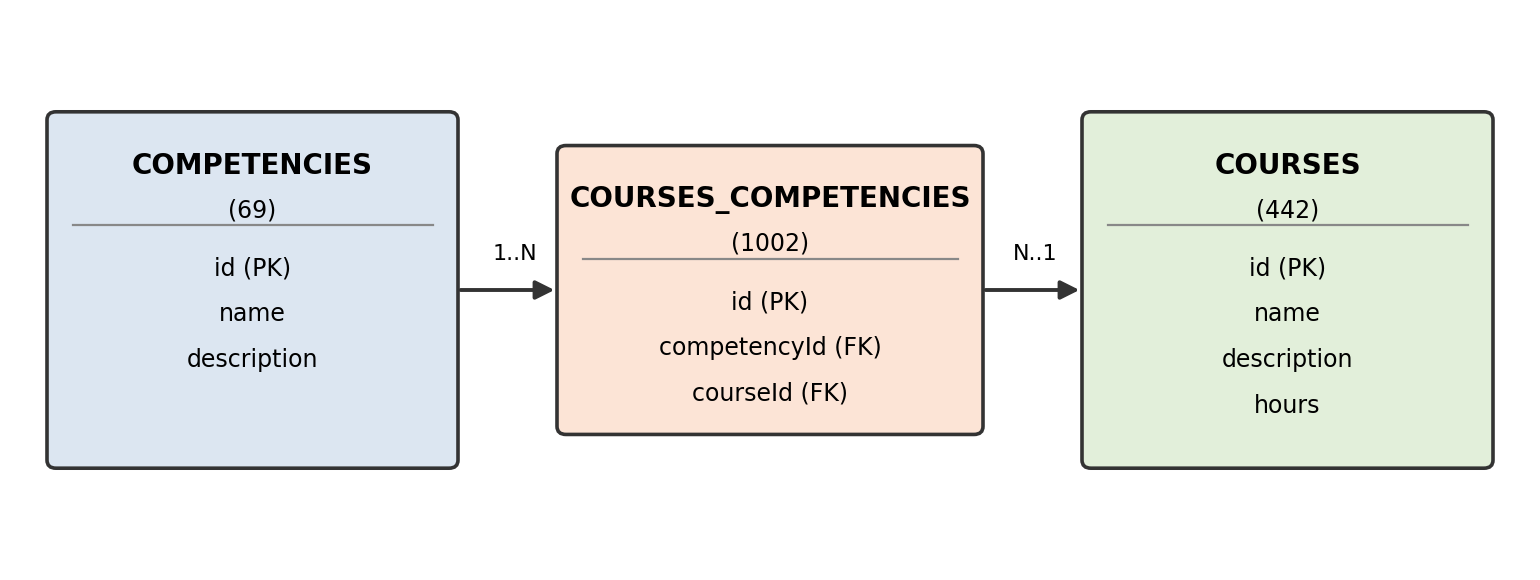
\includegraphics[width=0.85\textwidth]{paper/figures/fig_data_schema.png}
\caption{Entity-relationship diagram of the curation database, with row counts for the exported PlaforEdu catalog.}
\label{fig:schema}
\end{figure*}

\subsection{Agentic Workflow}
\label{subsec:agentic_layer}
We frame agentic curation as a directed cyclic graph compiled with LangGraph \cite{b_langgraph}, which guarantees structured, inspectable transitions between agents (Figure~\ref{fig:graph_flow}). The execution state carries $o_k$, the competency identifier, $A_k$, the current path $P_k$, and the critic's verdict and feedback.

\subsubsection{Context Node}
The entry node queries SQLite for the descriptor of the target competency and all candidate courses $A_k$.

\subsubsection{Generator Node}
Acting as an expert curator, this node receives $o_k$ and $A_k$, each course with its identifier, name and description, and outputs a sequence of selected courses with a pedagogical justification for each. Structured decoding with Pydantic schemas \cite{b_pydantic} guarantees machine-parseable output, but not that the identifiers it contains exist.

\subsubsection{Critic Node}
An independent critic reviews the path against two rules: the sequence must align with $o_k$, and it must contain at least three courses. It returns a binary verdict, ``Bom'' (good) or ``Ruim'' (bad), with natural-language feedback, following the self-reflection paradigm \cite{b_reflexion,b_selfrefine}.

\subsubsection{Routing}
If the verdict is ``Ruim'' and the budget is not exhausted, the graph routes back to the generator, injecting the feedback into its prompt; otherwise it terminates. We cap the workflow at three generator calls per competency.

\begin{figure}[t]
\centering
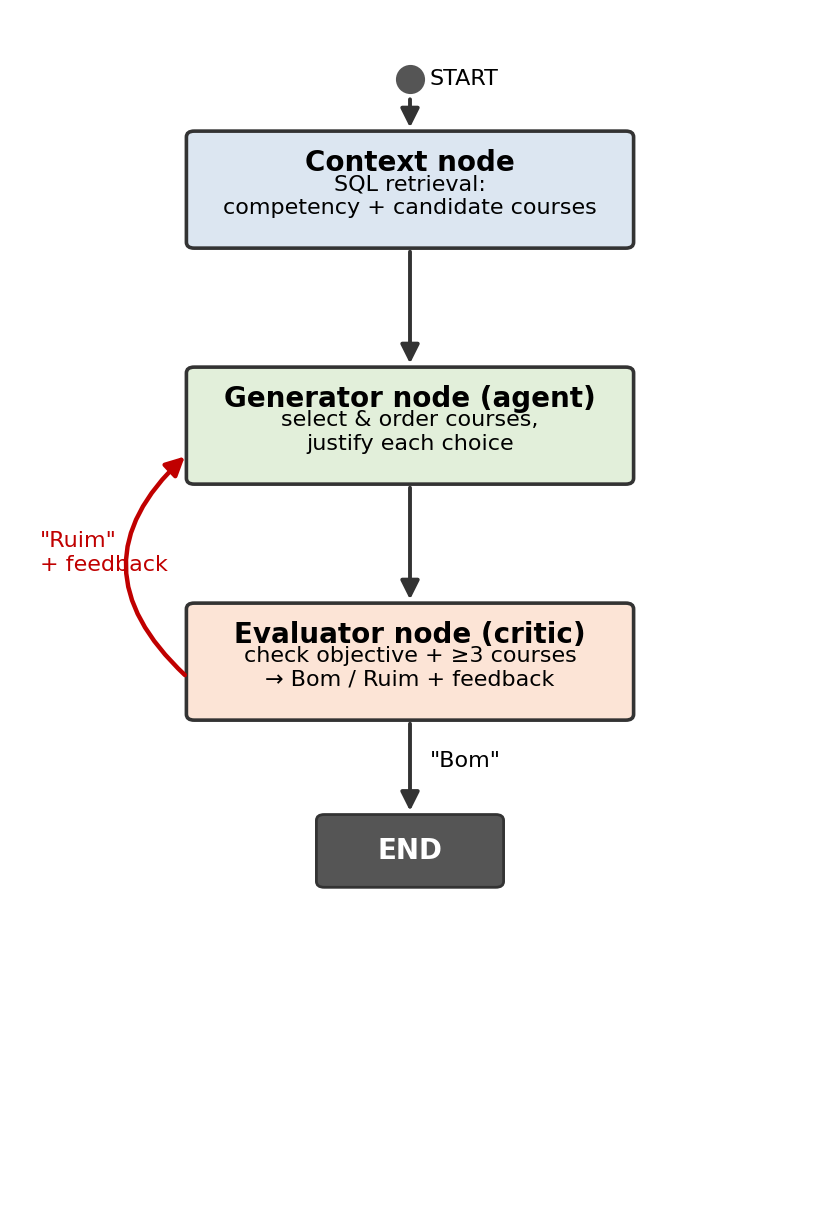
\includegraphics[width=0.82\linewidth]{paper/figures/fig_langgraph_flow.png}
\caption{State graph of the multi-agent curation workflow. Nodes are LLM agents and data extractors, and the red edge is the self-reflective refinement loop triggered by a ``Ruim'' verdict.}
\label{fig:graph_flow}
\end{figure}

\subsection{Guardrails and the Hybrid Design}
\label{subsec:guardrails}
Our preliminary study found that the critic loop, faced with pools smaller than its three-course rule, drove the generator to invent courses. We therefore define two programmatic guardrails. The \emph{pool-aware constraint} replaces the critic's minimum length by $\min(3,|A_k|)$. The \emph{identifier-validation gate} runs after every generator call: an identifier in $A_k$ is kept, an invalid identifier whose course name matches a course in $A_k$ is repaired to that course, duplicates are removed, and anything else is dropped. The \emph{guarded} multi-agent system applies both inside the graph.

The \emph{hybrid retrieve-generate-verify} system replaces the critic loop entirely. Embedding retrieval (Section~\ref{subsec:retrieval}) shortlists the ten courses most similar to $o_k$; a single generator call selects, orders and justifies courses from the shortlist only; and the validation gate filters the result. If fewer than $\min(3,|A_k|)$ courses survive, the path is padded with the most similar remaining shortlisted courses, never with generated ones.

\subsection{Retrieval Baselines}
\label{subsec:retrieval}
The retrieval systems embed $o_k$ and each course, name and description, with \texttt{text-embedding-3-small} \cite{b_embed} and return the $k$ most cosine-similar courses in descending order of similarity, with $k \in \{3,5,10\}$. The \emph{naive} baseline returns all of $A_k$ in catalog order and represents an uncurated catalog dump.

\subsection{System One Curation}
\label{subsec:system_one}
System One models cannot produce a sequence directly, so we decompose curation into per-course typed decisions and assemble the path deterministically (Figure~\ref{fig:system_one}). For every candidate $c \in A_k$, the state is the objective $o_k$ together with the course name and description, and the model answers two questions in one forward pass, both posed in Portuguese: a \emph{noul} question, whether the course contributes directly to the competency, which yields a probability $p_c$; and a three-level \emph{score} question, whether the course belongs at the start, middle or end of a learning path, which yields an expected level $\ell_c \in [0,2]$. The \emph{threshold} variant keeps the courses with $p_c \geq 0.5$, pads to $\min(3,|A_k|)$ with the next most probable courses, and orders the result by $\ell_c$, breaking ties by $p_c$. The \emph{top-5} variant keeps the five most probable courses, which matches the length of retrieval with $k{=}5$ and isolates selection quality from length. Because every selected element is a catalog item, the pipeline cannot produce an invalid identifier.

Our client speaks the \texttt{/v1/systemone} wire protocol, so the same code drives the hosted Jev and the open-source servers. Jev was available only through a waitlist when the experiments were run, so we evaluate the two open models: \textbf{Kev-4B} \cite{b_palmer2026kev}, a Qwen3.5-4B base model with a rank-16 adapter and a pointer head, released under Apache-2.0 and reported within four points of Jev on new-source decisions, and \textbf{Laya} \cite{b_laya2026}, whose multilingual checkpoint uses the 322M-parameter mmBERT encoder \cite{b_marone2025mmbert} and covers more than 100 languages. We use both zero-shot, with their shipped calibration.

\begin{figure*}[t]
\centering
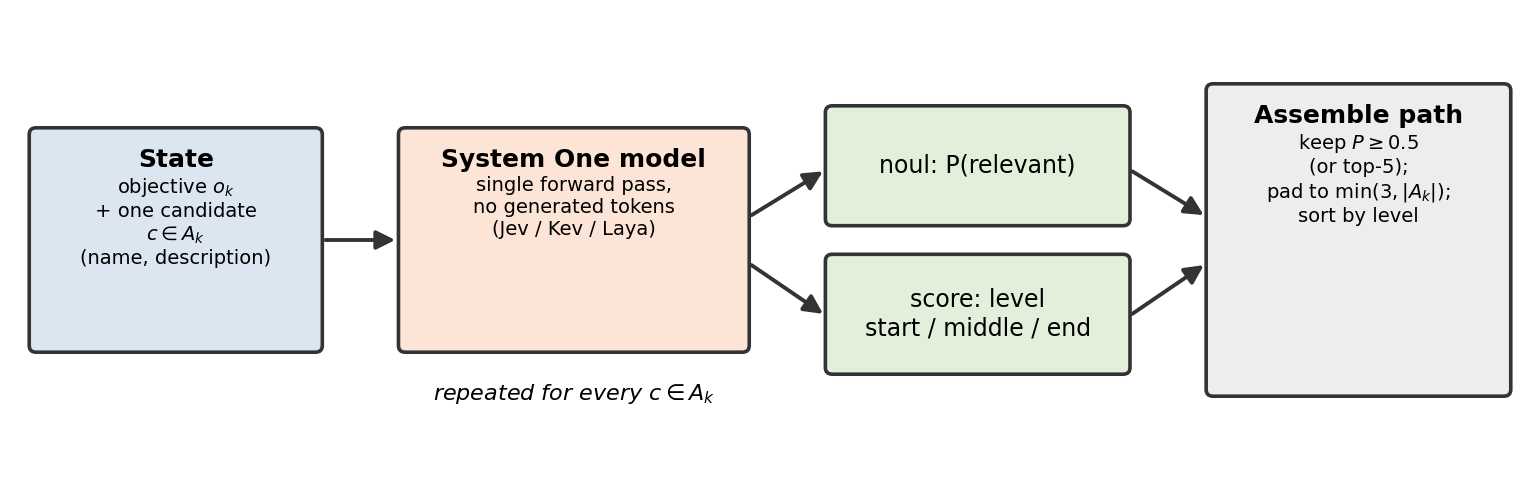
\includegraphics[width=0.85\textwidth]{paper/figures/fig_system_one.png}
\caption{System One curation. Each candidate course is scored independently by a non-autoregressive decision model with two typed questions, and the path is assembled by a fixed rule. No identifier is ever generated.}
\label{fig:system_one}
\end{figure*}

\section{Experimental Setup}
\label{sec:setup}

\subsection{Dataset}
We use the PlaforEdu catalog, the training platform of the Plan for Continuing Education of the servants of the Brazilian Federal Network of Professional, Scientific and Technological Education \cite{b_santos2025plafor}. It contains \RnCourses\ courses, \RnCompTotal\ competencies of which \RnCompCand\ have at least one candidate course, and \RnLinks\ course-competency associations. The number of candidates per competency is highly skewed, with a median of \RmedCand\ and a maximum of \RmaxCand\ (Figure~\ref{fig:dist}), so some competencies offer a rich pool to curate while a few offer fewer courses than the minimum length. We evaluate on the \RnComp\ competencies with candidate courses that the preliminary study processed, and every system is run on all of them so that comparisons are paired.

\begin{figure}[t]
\centering
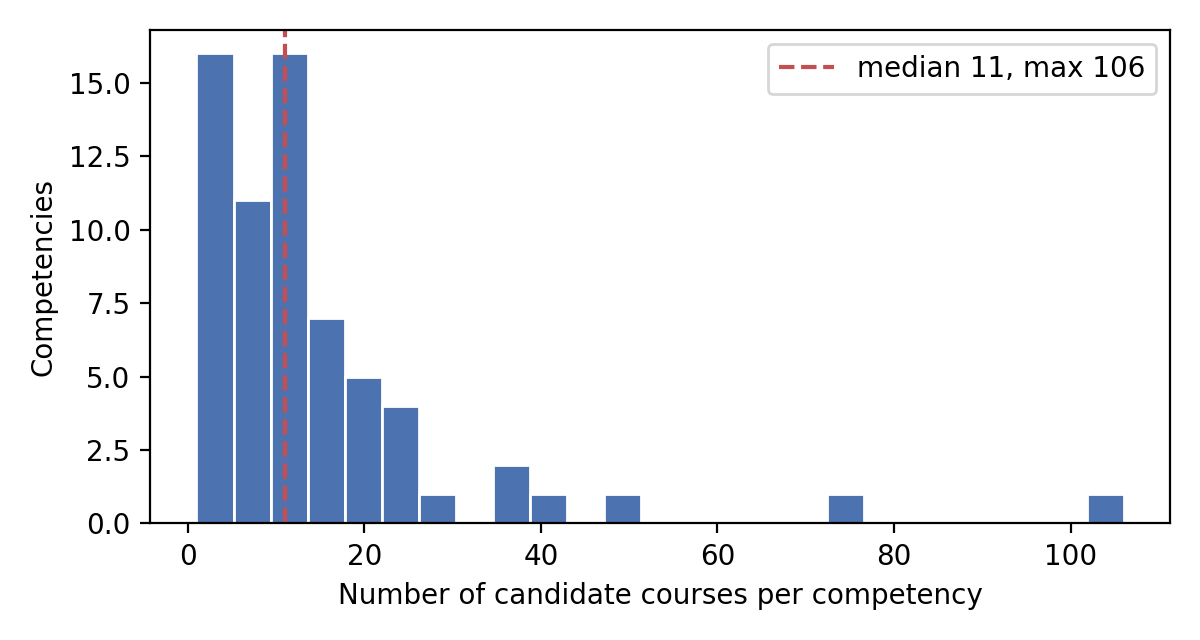
\includegraphics[width=\linewidth]{paper/figures/fig_courses_per_comp.png}
\caption{Distribution of candidate courses per competency in PlaforEdu.}
\label{fig:dist}
\end{figure}

\subsection{Systems Compared}
Table~\ref{tab:systems} lists the \VnVariants\ configurations. The LLM systems use one of three generators: \texttt{gpt-4o-mini}, the generator of the preliminary study, at temperature 0; and \texttt{gpt-5.4-mini}, a reasoning model, either with reasoning disabled (effort \texttt{none}), which we call \emph{System-1 operation}, or at effort \texttt{high}, which we call \emph{System-2 operation}. Critic and generator share the model within a configuration. The \emph{single agent} is the generator node alone, that is the multi-agent system with the critic ablated, and \emph{single agent, max.\ 5} adds the instruction to select at most five courses, a length control.

\begin{table}[t]
\centering
\caption{The compared system configurations. ``LLM calls'' counts generator and critic calls per path; ``Gen.\ IDs'' indicates whether the system emits identifiers that may be invalid.}
\label{tab:systems}
\footnotesize
\setlength{\tabcolsep}{3pt}
\begin{tabular}{llcc}
\toprule
System & Selector & LLM calls & Gen.\ IDs \\
\midrule
Naive dump & none & 0 & no \\
Retrieval, $k \in \{3,5,10\}$ & embeddings & 0 & no \\
Laya / Kev-4B, threshold & System One & 0 & no \\
Laya / Kev-4B, top-5 & System One & 0 & no \\
\midrule
Single agent & LLM & 1 & yes \\
Single agent, max.\ 5 & LLM & 1 & yes \\
Multi-agent (critic loop) & LLM & 2--6 & yes \\
Multi-agent, guarded & LLM + gate & 2--6 & gated \\
Hybrid retrieve-generate-verify & emb.\ + LLM + gate & 1 & gated \\
\bottomrule
\multicolumn{4}{l}{\parbox{0.95\linewidth}{\vspace{2pt}LLM systems run with \texttt{gpt-4o-mini}; single and multi-agent also with \texttt{gpt-5.4-mini} at reasoning effort \texttt{none} and \texttt{high}.}}
\end{tabular}
\end{table}

\subsection{Evaluation Protocol}
\label{subsec:protocol}
\subsubsection{Programmatic Metrics}
Computed without any model: path length $m$, the selection ratio $m/|A_k|$, the minimum-length satisfaction rate, duplicates, and the invalid-identifier rate, the fraction of selected courses not in $A_k$. We split invalid identifiers into \emph{corrupted}, whose course name exists in the catalog, and \emph{fabricated}, whose course does not exist at all.

\subsubsection{Judge Design}
The preliminary study's judge scored relevance, ordering, coverage and an overall grade in one call, without reasoning first and without seeing the candidate pool. Its diagnostics were poor: the overall score equalled the coverage score on \RpctCovEq\% of paths, relevance and ordering correlated at $\rho=\RrhoRelOrd$, \RpctThree\% of overall scores were exactly 3, and shorter paths scored higher ($\rho=\RrhoRatio$ between selection ratio and score). The redesigned judge addresses each issue. It sees the full candidate pool, so that coverage is judged against the courses actually available. It writes a short analysis citing courses \emph{before} each score, following G-Eval \cite{b_liu2023geval}. Each of five dimensions, relevance, coverage, ordering, concision and overall, has explicit anchors for every level from 1 to 5, and concision, the absence of redundant or superfluous courses, is separated from coverage so that length enters the rubric explicitly in both directions. Courses outside $A_k$ are shown as non-existent and anchored as severe relevance errors, and an empty path receives the minimum score on every dimension.

\subsubsection{Two Judge Families}
Two judges from different providers score every path: \texttt{gpt-4o} at temperature 0 and \texttt{claude-opus-5-5} at low reasoning effort, both with schema-constrained output. A judge from a family different from the generators bounds self-preference \cite{b_panickssery2024selfpref}, and the pair forms a small jury \cite{b_verga2024juries}. Our primary score is the mean of the two judges' overall scores. Neither judge is told which system produced a path.

\subsubsection{Statistical Analysis}
Competencies are the unit of analysis. For each configuration and competency we average the scores over runs, report the mean over competencies with a percentile-bootstrap $95\%$ confidence interval \cite{b_efron1993bootstrap}, and test fifteen \emph{planned} paired comparisons, one per research question component, with the two-sided Wilcoxon signed-rank test \cite{b_wilcoxon1945} using Pratt's treatment of zero differences, adjusting all fifteen $p$-values together with the Holm procedure \cite{b_holm}. As a complementary model-based analysis we fit a linear mixed-effects model with configuration as fixed effect and a random intercept per competency on the run-level scores \cite{b_bates2015lme4}. Inter-judge agreement is reported as Krippendorff's ordinal $\alpha$ \cite{b_hayes2007alpha}, quadratic-weighted $\kappa$ \cite{b_cohen1968kappa}, Spearman correlation and exact agreement.

\subsection{Implementation Details}
LLM systems were run three times per competency (runs 0--2); the deterministic systems, naive, retrieval with $k{=}5$ and System One, once. The \texttt{gpt-4o-mini} runs 0 of the single and multi-agent systems are those of the preliminary study and were re-judged with the new protocol. System One models were served locally on a single consumer GPU (NVIDIA RTX 3060, 12\,GB), Laya through its \texttt{laya-serve} server and Kev-4B in bfloat16 through \texttt{kev.serve}, and queried sequentially, one course per request. All prompts and System One questions are in Portuguese, matching the catalog. The workflow is implemented in Python with LangGraph \cite{b_langgraph} and Pydantic \cite{b_pydantic}. In total the study comprises \VnPaths\ generated paths and \VnJudgments\ judgments. One generation, a guarded multi-agent run on the largest pool, failed reproducibly because \texttt{gpt-4o-mini} entered a repetition loop until the 16{,}384-token output limit; we record it as an empty path, which is what a deployed system would return. Code, prompts, raw outputs, judgments and the analysis scripts that generate every number in this paper are released with the paper.\footnote{\url{https://github.com/silvaan/plafor-learning-paths}}

\section{Results}
\label{sec:results}
Table~\ref{tab:main2} reports quality, constraint and cost metrics for every configuration, Figure~\ref{fig:forest} summarizes overall quality with confidence intervals, and Table~\ref{tab:pairwise2} reports the planned comparisons.

\begin{table*}[t]
\centering
\caption{Main results over all competencies. Overall is the mean of the two v2 judges (gpt-4o, G; claude-opus-5-5, C), averaged over runs per competency, with a bootstrap 95\% CI. Rel., Cov., Ord.\ and Conc.\ are the per-dimension means of both judges. $m$ is the mean path length, Inv.\ the invalid-identifier rate over all runs, and Cost the generation cost per path in USD.}
\label{tab:main2}
\setlength{\tabcolsep}{3pt}
\footnotesize
\resizebox{\textwidth}{!}{%
\begin{tabular}{llccccccccccr}
\toprule
Family & System & Runs & Overall [95\% CI] & G & C & Rel. & Cov. & Ord. & Conc. & $m$ & Inv.\,\% & Cost \\
\midrule
Baseline & Naive dump & 1 & 2.17 [2.00, 2.33] & 3.20 & 2.17 & 2.32 & 4.80 & 2.23 & 1.85 & 15.0 & 0.0 & 0.00000 \\
\midrule
Retrieval & Retrieval, $k{=}3$ & 3 & 2.92 [2.73, 3.11] & 3.96 & 2.92 & 3.42 & 3.07 & 3.42 & 3.93 & 2.9 & 0.0 & 0.00000 \\
 & Retrieval, $k{=}5$ & 1 & 2.95 [2.77, 3.14] & 3.92 & 2.95 & 3.14 & 3.58 & 3.06 & 3.29 & 4.6 & 0.0 & 0.00000 \\
 & Retrieval, $k{=}10$ & 3 & 2.62 [2.47, 2.76] & 3.51 & 2.62 & 2.65 & 4.21 & 2.60 & 2.46 & 8.0 & 0.0 & 0.00000 \\
\midrule
System One & Laya, threshold & 1 & 2.27 [2.14, 2.41] & nan & 2.27 & 2.42 & 4.02 & 2.17 & 2.20 & 12.2 & 0.0 & 0.00000 \\
 & Laya, top-5 & 1 & 2.26 [2.09, 2.42] & nan & 2.26 & 2.47 & 2.91 & 2.38 & 2.88 & 4.6 & 0.0 & 0.00000 \\
 & Kev-4B, threshold & 1 & 2.89 [2.70, 3.09] & nan & 2.89 & 2.97 & 3.89 & 3.00 & 2.92 & 8.8 & 0.0 & 0.00000 \\
 & Kev-4B, top-5 & 1 & 3.03 [2.82, 3.26] & nan & 3.03 & 3.29 & 3.58 & 3.24 & 3.33 & 4.6 & 0.0 & 0.00000 \\
\midrule
LLM, gpt-4o-mini & Single agent & 3 & 2.79 [2.62, 2.95] & 3.69 & 2.79 & 2.75 & 4.19 & 3.02 & 2.68 & 7.7 & 0.5 & 0.00064 \\
 & Single agent, max.\ 5 & 3 & 3.11 [2.91, 3.29] & 4.18 & 3.11 & 3.21 & 3.73 & 3.37 & 3.51 & 4.6 & 0.5 & 0.00052 \\
 & Multi-agent (critic loop) & 3 & 2.80 [2.64, 2.96] & 3.74 & 2.80 & 2.73 & 4.15 & 3.05 & 2.64 & 7.6 & 3.3 & 0.00085 \\
 & Multi-agent, guarded & 3 & 2.83 [2.66, 2.99] & 3.81 & 2.83 & 2.83 & 4.13 & 3.03 & 2.73 & 7.5 & 0.0 & 0.00088 \\
 & Hybrid retrieve-generate-verify & 3 & 2.87 [2.69, 3.05] & nan & 2.87 & 2.90 & 4.17 & 3.03 & 2.75 & 7.1 & 0.0 & 0.00051 \\
\midrule
LLM, gpt-5.4-mini, no reasoning & Single agent & 3 & 3.25 [3.09, 3.40] & nan & 3.25 & 3.21 & 4.07 & 3.59 & 3.34 & 5.9 & 0.9 & 0.00367 \\
 & Multi-agent (critic loop) & 3 & 3.25 [3.07, 3.41] & nan & 3.25 & 3.15 & 4.07 & 3.52 & 3.25 & 6.0 & 0.7 & 0.00536 \\
\midrule
LLM, gpt-5.4-mini, high reasoning & Single agent & 3 & 3.61 [3.43, 3.78] & 1.00 & 3.61 & 3.53 & 4.03 & 4.05 & 3.84 & 5.2 & 0.4 & 0.01414 \\
 & Multi-agent (critic loop) & 3 & 3.48 [3.30, 3.66] & 1.00 & 3.48 & 3.41 & 4.05 & 3.97 & 3.73 & 5.4 & 0.8 & 0.02026 \\
\bottomrule
\end{tabular}}
\end{table*}


\begin{figure}[t]
\centering
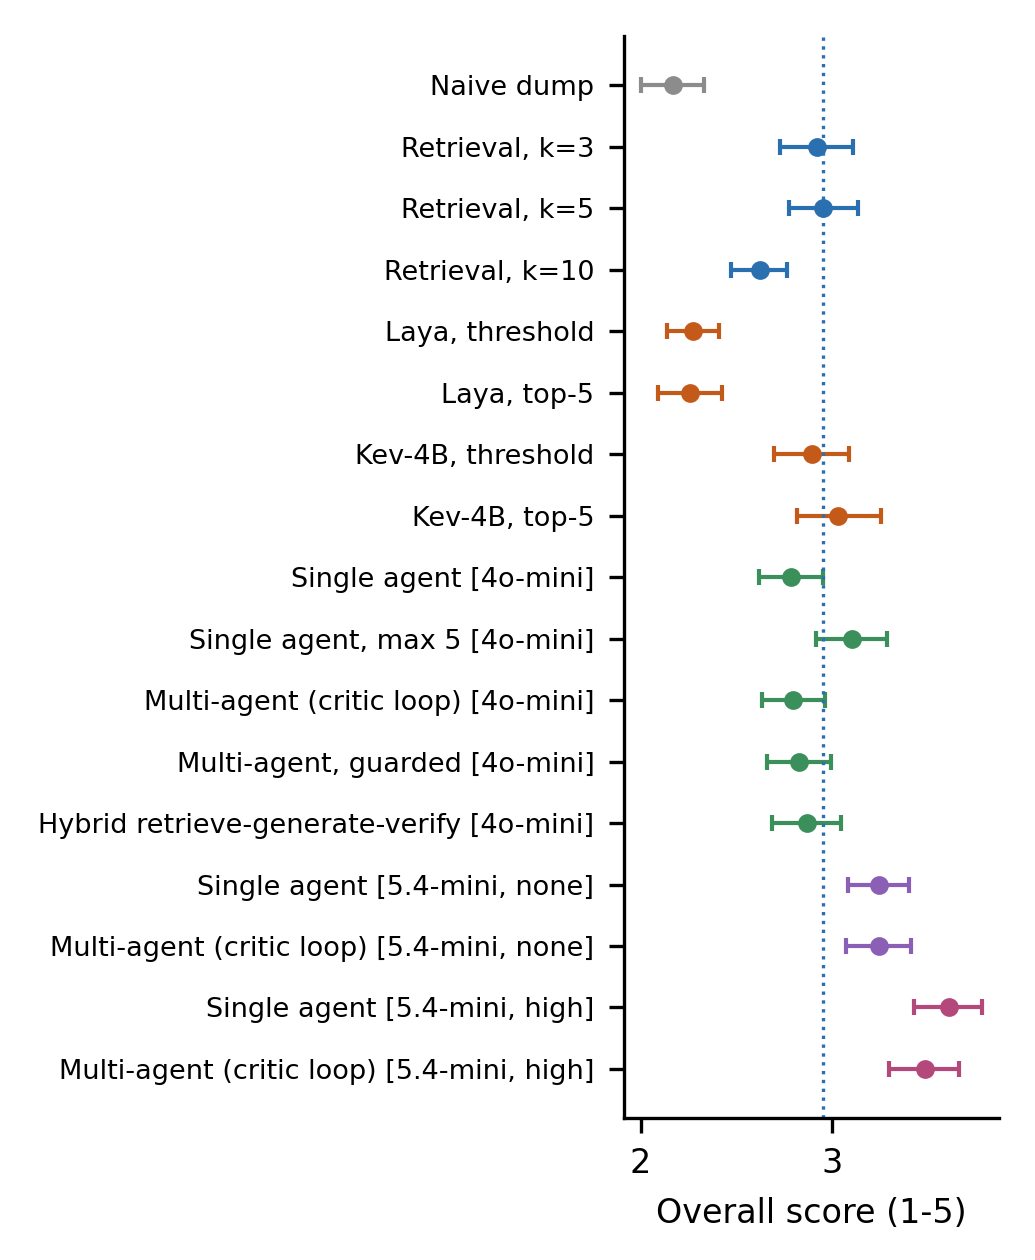
\includegraphics[width=\linewidth]{paper/figures/fig2_forest.png}
\caption{Overall score per configuration, mean of the two judges with bootstrap 95\% confidence intervals over the \RnComp\ competencies. The dotted line marks embedding retrieval with $k{=}5$. Colours denote system families.}
\label{fig:forest}
\end{figure}

\begin{table*}[t]
\centering
\caption{Planned paired comparisons on the per-competency mean overall score (primary judge, runs averaged). $\Delta$ is A minus B with a bootstrap 95\% CI; W/T/L counts competencies where A wins, ties or loses; $p_{\mathrm{Holm}}$ is the Wilcoxon signed-rank $p$-value, Holm-adjusted over all comparisons.}
\label{tab:pairwise2}
\footnotesize
\begin{tabular}{lllcccr}
\toprule
Question & A & B & $\Delta$ [95\% CI] & W/T/L & $n$ & $p_{\mathrm{Holm}}$ \\
\midrule
retrieval vs. proposed multi-agent & Retrieval $k{=}5$ & Multi-agent (4o-mini) & +0.16 [+0.02, +0.30] & 22/30/14 & 66 & 0.727 \\
critic loop, gpt-4o-mini & Single (4o-mini) & Multi-agent (4o-mini) & -0.01 [-0.09, +0.07] & 13/38/15 & 66 & 1.000 \\
guardrails on the loop & Multi-agent (4o-mini) & Guarded (4o-mini) & -0.03 [-0.11, +0.04] & 13/39/14 & 66 & 1.000 \\
hybrid vs. retrieval & Hybrid (4o-mini) & Retrieval $k{=}5$ & -0.09 [-0.20, +0.03] & 10/39/17 & 66 & 1.000 \\
hybrid vs. multi-agent & Hybrid (4o-mini) & Multi-agent (4o-mini) & +0.07 [-0.04, +0.18] & 20/32/14 & 66 & 1.000 \\
length cap on the single agent & Single (4o-mini) & Single max.\,5 (4o-mini) & -0.32 [-0.43, -0.21] & 5/22/39 & 66 & <0.001 \\
reasoning, single agent & Single (5.4, none) & Single (5.4, high) & -0.36 [-0.47, -0.25] & 6/18/42 & 66 & <0.001 \\
reasoning, multi-agent & Multi-agent (5.4, none) & Multi-agent (5.4, high) & -0.24 [-0.33, -0.14] & 7/26/33 & 66 & <0.001 \\
critic loop under high reasoning & Single (5.4, high) & Multi-agent (5.4, high) & +0.13 [+0.07, +0.19] & 24/36/6 & 66 & 0.007 \\
critic loop without reasoning & Single (5.4, none) & Multi-agent (5.4, none) & -0.00 [-0.10, +0.10] & 15/31/20 & 66 & 1.000 \\
System One (Kev) vs. retrieval & Kev-4B thr. & Retrieval $k{=}5$ & -0.06 [-0.26, +0.14] & 16/32/18 & 66 & 1.000 \\
System One (Laya) vs. retrieval & Laya thr. & Retrieval $k{=}5$ & -0.68 [-0.86, -0.50] & 1/29/36 & 66 & <0.001 \\
Kev top-5 vs. retrieval at equal length & Kev-4B top-5 & Retrieval $k{=}5$ & +0.08 [-0.09, +0.24] & 16/38/12 & 66 & 1.000 \\
System One vs. System-1 LLM & Kev-4B thr. & Single (5.4, none) & -0.35 [-0.53, -0.18] & 14/19/33 & 66 & 0.008 \\
selection vs. no selection & Naive dump & Retrieval $k{=}5$ & -0.79 [-0.98, -0.59] & 2/24/40 & 66 & <0.001 \\
\bottomrule
\end{tabular}
\end{table*}


\subsection{Selection Matters, and Retrieval Is a Strong Baseline}
\label{subsec:baselines}
Selecting courses clearly beats dumping the catalog. The naive dump scores \VovNaive\ against \VovRetr\ for retrieval with $k{=}5$, a difference of $\VdNaiveRetr$ (win/tie/loss for the dump \VwlNaiveRetr, $p_{\mathrm{Holm}}\VpNaiveRetr$). The dump scores the maximum on coverage, \VcovNaive, because it contains every candidate, but collapses on concision, \VconNaive, and ordering, \VordNaive, exactly the trade-off the new rubric was designed to expose. Among the retrieval variants, $k{=}3$ and $k{=}5$ are statistically indistinguishable, at \VovRetrThree\ and \VovRetr, while $k{=}10$ drops to \VovRetrTen. Against this baseline, the \texttt{gpt-4o-mini} systems of the preliminary study do not improve: retrieval leads the proposed multi-agent system by $\VdRetrMulti$ ($95\%$ CI $[\VdloRetrMulti, \VdhiRetrMulti]$, $p_{\mathrm{Holm}}\VpRetrMulti$), confirming with two new judges and three runs the direction of the preliminary result, though the gap is no longer significant after correction.

\subsection{RQ1: The Critic Loop and Its Guardrails}
\label{subsec:loop}
The critic loop does not improve paths. With \texttt{gpt-4o-mini}, the multi-agent and single-agent systems differ by $\VdSingleMulti$ ($p_{\mathrm{Holm}}\VpSingleMulti$, win/tie/loss \VwlSingleMulti), and with \texttt{gpt-5.4-mini} without reasoning by $\VdSingleNoneMultiNone$ ($p_{\mathrm{Holm}}\VpSingleNoneMultiNone$). The loop rarely activates: the critic rejected the first path on \VfiredMulti\% of \texttt{gpt-4o-mini} runs, \VfiredSmallMulti\ of the \VfiredNMulti\ activations on pools smaller than three courses, where no valid path can satisfy its rule, and on \VfiredMultiNone\% of non-reasoning \texttt{gpt-5.4-mini} runs.

It is exactly there that the loop is harmful. Table~\ref{tab:halluc2} shows that fabricated courses, courses that do not exist anywhere in the catalog, occur in \emph{one} configuration only, the unguarded \texttt{gpt-4o-mini} multi-agent system, with \VhalFabMulti\ fabricated courses, all on competencies whose pool is smaller than the three-course rule: rejected for being honestly short, the generator complied by inventing plausible titles, and the critic then approved them. Corrupted identifiers, real courses with a rewritten identifier, are an ordinary structured-output error that affects every LLM configuration at a low rate, including the reasoning model. The guardrails remove both. The guarded multi-agent system produced no invalid identifier at all, \VhalPathsGuard\ affected paths out of \VrunsNGuard, its gate repairing or dropping \VgateFixesGuard\ entries along the way, its critic firing on only \VfiredNGuard\ runs, and its quality is indistinguishable from the unguarded loop ($\VdMultiGuard$, $p_{\mathrm{Holm}}\VpMultiGuard$). The hybrid design, which needs no critic at all, likewise has no invalid identifier and matches both retrieval ($\VdHybridRetr$, $p_{\mathrm{Holm}}\VpHybridRetr$) and the multi-agent system ($\VdHybridMulti$, $p_{\mathrm{Holm}}\VpHybridMulti$).

\begin{table}[t]
\centering
\caption{Invalid identifiers over all generated paths (every run). Corrupted: the name exists in the catalog but the identifier is not in $A_k$. Fabricated: the course does not exist. Systems not listed produced none.}
\label{tab:halluc2}
\footnotesize
\begin{tabular}{lrrrr}
\toprule
System & Paths & Affected & Corr. & Fabr. \\
\midrule
Single (4o-mini) & 198 & 11 & 11 & 0 \\
Single max.\,5 (4o-mini) & 198 & 5 & 5 & 0 \\
Multi-agent (4o-mini) & 198 & 18 & 13 & 16 \\
Single (5.4, none) & 198 & 12 & 12 & 0 \\
Multi-agent (5.4, none) & 198 & 9 & 9 & 0 \\
Single (5.4, high) & 198 & 7 & 7 & 0 \\
Multi-agent (5.4, high) & 198 & 11 & 11 & 0 \\
\bottomrule
\end{tabular}
\end{table}


The answer to RQ1 is therefore that the critic adds cost, \VitersMulti\ generator calls on average plus one critic call per iteration, and a fabrication risk, but no quality, and that a few lines of programmatic verification achieve what the critic was meant to achieve, valid paths of adequate length, more reliably.

\subsection{RQ2: System-1 Versus System-2 Generation}
\label{subsec:reasoning}
Explicit reasoning is the only intervention in our study that clearly improves curation. With the \emph{same} model, \texttt{gpt-5.4-mini}, switching reasoning from \texttt{none} to \texttt{high} raises the single-agent score from \VovSingleNone\ to \VovSingleHigh\ ($\VdSingleNoneSingleHigh$ for none minus high, CI $[\VdloSingleNoneSingleHigh, \VdhiSingleNoneSingleHigh]$, win/tie/loss \VwlSingleNoneSingleHigh, $p_{\mathrm{Holm}}\VpSingleNoneSingleHigh$) and the multi-agent score from \VovMultiNone\ to \VovMultiHigh\ ($p_{\mathrm{Holm}}\VpMultiNoneMultiHigh$). The gain is concentrated on the dimensions where planning should matter. Ordering rises from \VordSingleNone\ to \VordSingleHigh\ and concision from \VconSingleNone\ to \VconSingleHigh, while coverage is unchanged, \VcovSingleNone\ against \VcovSingleHigh, and the reasoning paths are slightly shorter, \VnselSingleHigh\ against \VnselSingleNone\ courses. The reasoning model thus selects similar material but sequences it more coherently and prunes redundancy. Even without reasoning, the newer model already outscores \texttt{gpt-4o-mini}, \VovSingleNone\ against \VovSingle, so model generation and reasoning effort contribute separately (Figure~\ref{fig:reasoning}).

Reasoning also changes the value of the critic, for the worse. Under high reasoning the critic rejected the first path on \VfiredMultiHigh\% of runs, far more often than without reasoning, yet the single agent \emph{outscores} the multi-agent system by $\VdSingleHighMultiHigh$ (CI $[\VdloSingleHighMultiHigh, \VdhiSingleHighMultiHigh]$, win/tie/loss \VwlSingleHighMultiHigh, $p_{\mathrm{Holm}}\VpSingleHighMultiHigh$). A deliberate generator does not need a critic to satisfy two simple rules, and the critic's feedback, which concerns only alignment and minimum length, displaces paths that the generator had already reasoned about. The cost of the best configuration remains small, \$\VcostSingleHigh\ and \VlatSingleHigh\,s per path.

\begin{figure}[t]
\centering
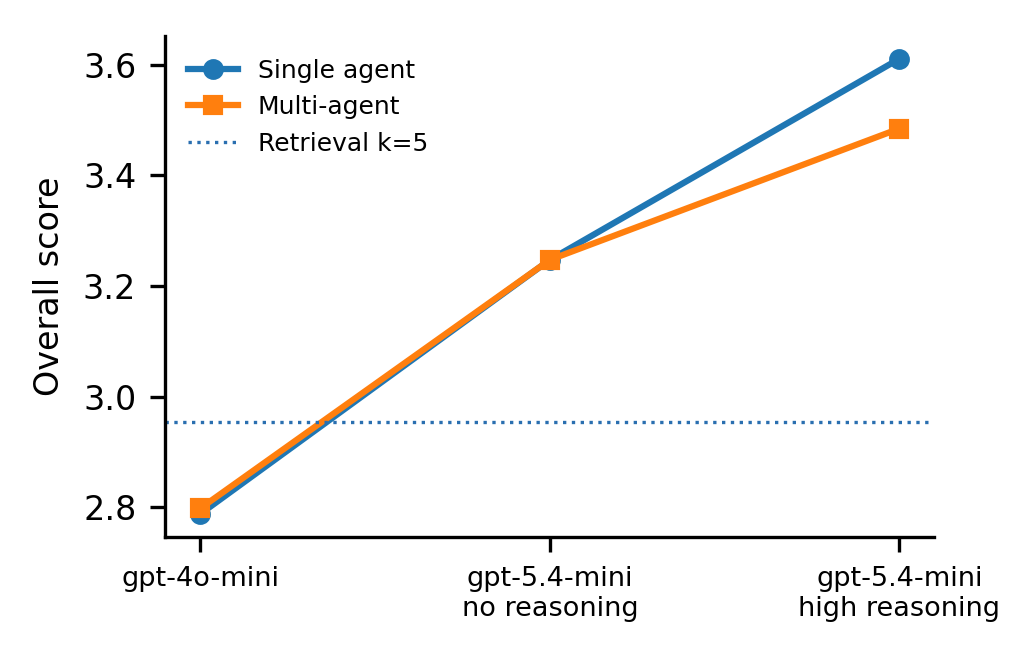
\includegraphics[width=\linewidth]{paper/figures/fig2_reasoning.png}
\caption{Overall score by generator and architecture. Reasoning raises quality for both architectures, and under high reasoning the critic loop scores below the single agent. The dotted line marks retrieval with $k{=}5$.}
\label{fig:reasoning}
\end{figure}

\subsection{RQ3: System One Decision Models}
\label{subsec:s1results}
The two System One models behave very differently. Kev-4B is competitive with embedding retrieval: \VovKev\ for the threshold variant and \VovKevFive\ for the top-5 variant, against \VovRetr\ for retrieval with $k{=}5$ ($p_{\mathrm{Holm}}\VpKevRetr$ and $\VpKevFiveRetr$, win/tie/loss \VwlKevFiveRetr\ at equal length). Its relevance probabilities are informative: over all candidate courses they predict whether the high-reasoning LLM selected a course with an area under the ROC curve of \VaucKev, and \VpAboveKev\% of candidates pass the 0.5 threshold. It does not, however, reach the generative LLMs; it trails the non-reasoning \texttt{gpt-5.4-mini} single agent by $\VdKevSingleNone$ ($p_{\mathrm{Holm}}\VpKevSingleNone$). Its ordering by predicted level is no better than retrieval's similarity order, \VordKevFive\ against \VordRetr.

Laya, in contrast, fails on this task: \VovLaya\ and \VovLayaFive\ for the two variants, no better than the naive dump ($p_{\mathrm{Holm}}\VpLayaRetr$ against retrieval). Its relevance probabilities are nearly uninformative, with an AUC of \VaucLaya\ and \VpAboveLaya\% of all candidates judged relevant, including, for instance, a course for teaching assistants under a strategic-vision competency. Laya's shipped heads were trained on routing-style decisions over short texts, and judging the pedagogical fit of a course to a competency in Portuguese is far from that distribution. The contrast suggests that, at the current state of the art, the decision quality of System One models comes from the backbone, a 4B-parameter generative base model for Kev against a 322M-parameter encoder for Laya, more than from the non-autoregressive interface.

Cost and speed favour System One models in principle but depend on deployment. Laya took \(0.08\)\,s per candidate course on our consumer GPU; Kev-4B took about 2.3\,s per candidate, sequentially, so that a large pool took tens of seconds, whereas its developers report tens of milliseconds per request on data-centre GPUs with batching \cite{b_palmer2026kev}. Neither incurs any per-token API cost, and neither can produce an invalid identifier. For a platform with data-sovereignty constraints, a locally served Kev-class model thus offers retrieval-level quality with an explicit, per-course, probabilistic rationale.

\subsection{RQ4: Path Length Confounds Comparisons}
\label{subsec:length}
Length explains a large part of the differences above. The single instruction ``select at most five courses'' raises the \texttt{gpt-4o-mini} single agent from \VovSingle\ to \VovSingleFive\ ($\VdSingleSingleFive$, $p_{\mathrm{Holm}}\VpSingleSingleFive$), more than any architectural change to that model and enough to overtake retrieval. In a regression of the overall score on configuration and the logarithm of path length, the length coefficient is \VbetaLogLen\ ($p\VpLogLen$), and the retrieval sweep shows a clear optimum at small $k$. Figure~\ref{fig:length} shows the mechanism in the rubric: as the selection ratio $m/|A_k|$ grows, coverage rises and concision falls for both judges, and the overall score follows concision more than coverage. Comparisons between systems that produce paths of different lengths, which includes most comparisons in the curation literature, therefore partly measure the length preference built into the rubric. The reasoning gain in Section~\ref{subsec:reasoning} survives this concern: the reasoning paths are only marginally shorter, and the high-reasoning single agent outscores the length-capped \texttt{gpt-4o-mini} agent at almost the same length.

\begin{figure}[t]
\centering
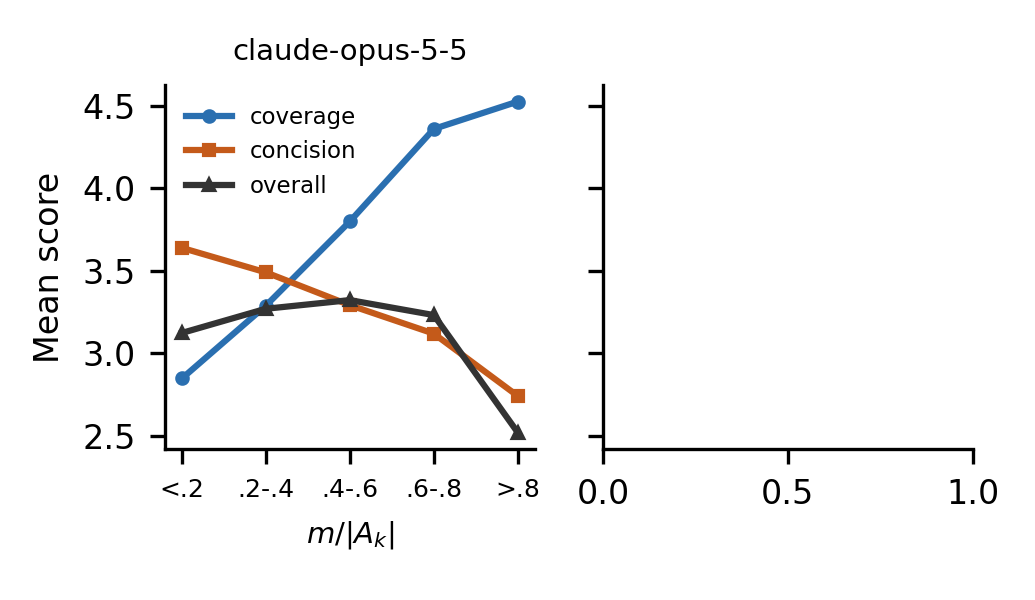
\includegraphics[width=\linewidth]{paper/figures/fig2_length.png}
\caption{Mean coverage, concision and overall scores by selection ratio $m/|A_k|$, for each judge, over all selective systems. Longer paths gain coverage and lose concision.}
\label{fig:length}
\end{figure}

\subsection{RQ5: How Reliable Are the Judges?}
\label{subsec:judge}
Table~\ref{tab:agree} reports the agreement between the two judges. On individual paths it is modest: Krippendorff's ordinal $\alpha$ is \ValphaOverall\ for the overall score and ranges from \ValphaOrdering\ for ordering to \ValphaConcision\ for concision, with Spearman correlations of \VrhoOrdering\ to \VrhoConcision. Part of the disagreement is a constant offset, since \texttt{gpt-4o} is systematically more lenient than \texttt{claude-opus-5-5}, which $\alpha$ and $\kappa$ penalize but $\rho$ does not. At the level that matters for conclusions, however, the judges agree almost perfectly: their mean overall scores per configuration correlate at Spearman $\rho=\VrhoSysJudges$ (Kendall $\tau=\VtauSysJudges$). We find no evidence of self-preference: the gap between the OpenAI judge and the Anthropic judge is \VgapOpenAI\ points on paths generated by OpenAI models and \VgapOther\ on paths from non-generative systems ($p\VpGap$).

\begin{table}[t]
\centering
\caption{Agreement between the two v2 judges over all judged paths: Krippendorff's ordinal $\alpha$, quadratic-weighted $\kappa$, Spearman $\rho$, exact agreement, and each judge's mean.}
\label{tab:agree}
\footnotesize
\begin{tabular}{lcccccc}
\toprule
Dimension & $\alpha$ & $\kappa_w$ & $\rho$ & Exact\,\% & G & C \\
\midrule
Relevance & 0.41 & 0.54 & 0.75 & 27 & 3.69 & 2.90 \\
Coverage & 0.38 & 0.41 & 0.39 & 43 & 3.91 & 3.94 \\
Ordering & 0.20 & 0.35 & 0.48 & 30 & 3.87 & 3.03 \\
Concision & 0.50 & 0.55 & 0.76 & 25 & 3.77 & 2.94 \\
Overall & 0.22 & 0.42 & 0.68 & 21 & 3.77 & 2.81 \\
\bottomrule
\end{tabular}
\end{table}


The redesigned rubric also removed the collapse of the preliminary judge. The overall score now equals the coverage score on \VpctOvEqCovG\% (\texttt{gpt-4o}) and \VpctOvEqCovC\% (\texttt{claude-opus-5-5}) of paths, against \RpctCovEq\% before; relevance and ordering are distinct dimensions for the Anthropic judge ($\rho=\VrhoRelOrdC$) though still entangled for the OpenAI judge ($\rho=\VrhoRelOrdG$); and coverage and concision pull in opposite directions with length, as intended. On the \VnVOne\ paths judged by both protocols, the old and new overall scores correlate only at $\rho=\VrhoVOneVTwo$, a reminder that absolute judge scores are protocol-specific and only within-protocol comparisons are meaningful.

\subsection{Decoding Variability}
\label{subsec:variability}
Repeated runs at fixed settings are far from deterministic, consistent with prior reports on LLM API nondeterminism \cite{b_nondeterminism}. Across the three runs, \texttt{gpt-4o-mini} produced the identical path for only \VidentSingle\% of competencies in the single-agent configuration and the same set of courses for \VsamesetSingle\%; for \texttt{gpt-5.4-mini}, whose reasoning variant ignores the temperature parameter, identical paths occurred for \VidentSingleNone\% (no reasoning) and \VidentSingleHigh\% (high reasoning) of competencies. The mean within-competency standard deviation of the overall score across runs is \VsdSingle\ to \VsdSingleNone\ points, of the same order as several between-system differences in Table~\ref{tab:pairwise2}. Single-run comparisons of LLM curators are therefore unreliable. The mixed model also shows that competencies differ systematically: the random intercept accounts for \VmmICC\ of the variance left after the configuration effects, which is why all our comparisons are paired by competency.

\subsection{Effect of Candidate-Pool Size}
\label{subsec:poolsize}
Figure~\ref{fig:by_size2} stratifies quality by pool size. With one or two candidates there is nothing to curate, and every system scores around \VovRetrBucketA. With three to five, no system is clearly better than the naive dump, because the dump already is a short path. The systems separate on pools of six or more courses: on the \VnBucketD\ competencies with more than ten candidates the high-reasoning single agent reaches \VovSingleHighBucketD, against \VovRetrBucketD\ for retrieval and \VovNaiveBucketD\ for the dump. The advantage of reasoning thus grows with the size of the selection problem, where both pruning and sequencing matter most.

\begin{figure}[t]
\centering
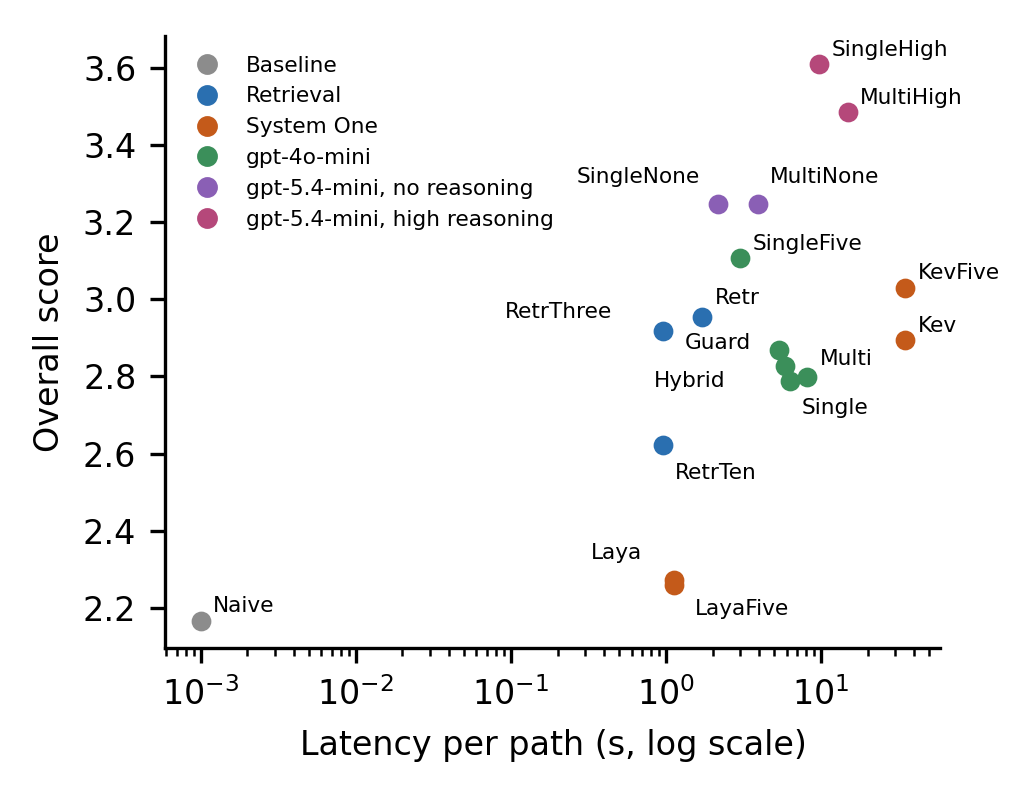
\includegraphics[width=\linewidth]{paper/figures/fig2_pareto.png}
\caption{Quality versus latency per path, log scale. System One latencies were measured on a consumer GPU with sequential per-course requests; the naive dump is plotted at 1\,ms. High-reasoning generation is the quality frontier, while retrieval and the length-capped single agent offer most of the quality at a fraction of the latency.}
\label{fig:pareto}
\end{figure}

\begin{figure}[t]
\centering
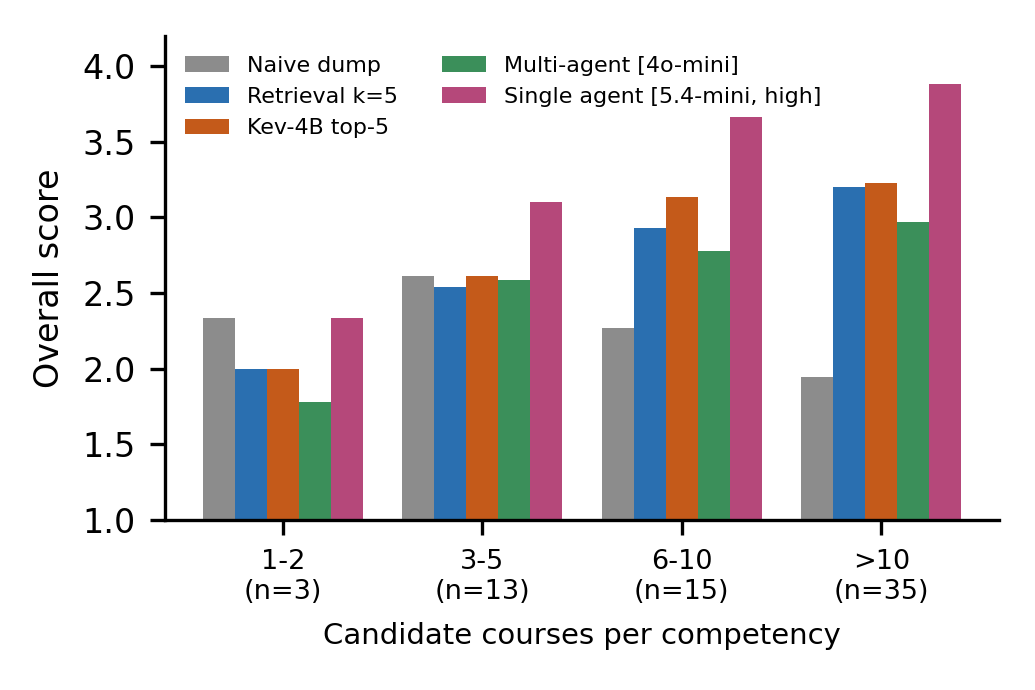
\includegraphics[width=\linewidth]{paper/figures/fig2_bysize.png}
\caption{Mean overall score by number of candidate courses for selected configurations, with the number of competencies per stratum.}
\label{fig:by_size2}
\end{figure}

\subsection{Efficiency}
\label{subsec:efficiency}
All systems are cheap compared with human curation, which takes hours per path. Retrieval needs one embedding call; the \texttt{gpt-4o-mini} systems cost about \$\VcostSingle\ to \$\VcostMulti\ per path; and the best configuration, the high-reasoning single agent, costs \$\VcostSingleHigh\ and \VlatSingleHigh\,s per path, while the high-reasoning multi-agent system costs more, \$\VcostMultiHigh\ and \VlatMultiHigh\,s, for lower quality (Figure~\ref{fig:pareto}). Across the whole study, generation cost \$\VgenCostTotal\ and judging \$\VjudgeCostTotal: evaluation, not generation, dominates the budget of a rigorous study of this kind.

\section{Discussion}
\label{sec:discussion}

\subsection{What Should a Platform Deploy?}
The results support a simple deployment rule. Where a hosted reasoning model is acceptable, a \emph{single} reasoning-model call constrained to catalog courses, followed by the identifier-validation gate and the pool-aware length rule, gives the best quality we observed at a cost of fractions of a cent per path, and needs no critic loop. Where data must stay on premises or cost must be near zero, embedding retrieval with a small $k$ or a locally served System One model of the Kev class gives a solid, hallucination-free baseline, and the System One model adds a per-course relevance probability that a human curator can audit or threshold. Regardless of the selector, programmatic verification is mandatory, because every generative configuration produced invalid identifiers at some rate, and because an LLM critic is not a substitute for it: the critic approved fabricated courses.

\subsection{Why Did the Critic Loop Fail?}
Self-refinement helps when the critic has information or checking ability that the generator lacks \cite{b_kamoi2024selfcorrect}. Our critic, faithful to the original architecture, checked a length rule and a vague alignment rule, neither of which supplies such information; the length rule is trivially checkable in code, and the alignment rule is something the generator already optimizes. The loop therefore either did nothing or, when it fired, pushed the generator towards the critic's narrow notion of quality, most visibly when the generator was already deliberating with a reasoning model and when the pool made the length rule unsatisfiable. This agrees with taxonomies of multi-agent failure, in which weak verification and misaligned specifications dominate \cite{b_cemri2025mas}. A critic worth its cost would need external signals, for example prerequisite relations \cite{b_liu2020prereq}, learner outcomes or curator feedback.

\subsection{Fast, Slow, or Agentic?}
The title's question has a clear answer on this task. \emph{Slow} thinking, explicit reasoning by the generator, improves curation, mostly by ordering courses into a coherent progression and pruning redundant ones. \emph{Agentic} structure, a separate critic, does not, and becomes counterproductive once the generator reasons. \emph{Fast} non-generative selection, by retrieval or by a capable System One model, does not reach reasoning-level quality, but it is a competitive, verifiable and cheap floor that any more complex system must clearly beat; the fact that the proposed multi-agent system of our preliminary study did not beat it illustrates why such baselines must be reported \cite{b_agents_matter}.

\subsection{Implications for Evaluating Curation Systems}
Three practices follow from RQ4 and RQ5. First, control or report path length, because a one-line length instruction moved scores more than any architecture; equal-length variants such as our top-5 System One and capped single agent make comparisons interpretable. Second, use repeated runs and paired, multiplicity-corrected tests, because temperature-0 decoding is not deterministic and run-to-run variation is of the same order as many reported gains. Third, use more than one judge and interpret them at the level of system rankings, where they agree, rather than individual paths, where they do not; and keep programmatic checks outside the judge, which in our preliminary study did not penalize courses explicitly labelled as non-existent.

\subsection{Threats to Validity}
\label{subsec:threats}
\textit{Construct validity.} Quality is measured by LLM judges. We mitigated known weaknesses with a reason-first, anchored, pool-aware rubric and two judges from different families, whose system rankings agree, but item-level agreement is modest and no human ratings are yet reported. We prepared a blind evaluation protocol in which curators score a stratified sample of 80 paths from five systems on the same rubric, released with the code, and its results are needed to anchor the absolute scale. \textit{Internal validity.} LLM systems were run three times and deterministic ones once; System One models were used zero-shot with their shipped calibration, and fine-tuning, which their developers report as the main lever for accuracy \cite{b_palmer2026kev,b_laya2026}, could change their standing; the System One questions were written once and not tuned. The hosted Jev was not available to us, so our System One conclusions concern its open-source counterparts. \textit{External validity.} Results concern one Portuguese-language public-sector catalog with \RnComp\ evaluable competencies, curation by textual descriptions only, and specific model versions; Laya's failure may be specific to Portuguese. \textit{Statistical conclusion validity.} The integer scale produces many ties, which reduces the power of signed-rank tests; we report win, tie and loss counts, bootstrap intervals, a mixed model, and Holm-adjusted $p$-values over fifteen planned comparisons.

\section{Conclusion}
\label{sec:conclusion}
We compared non-generative, generative and agentic approaches to curating learning paths on the full catalog of a Brazilian public-sector training platform, with \VnPaths\ paths from \VnVariants\ configurations, repeated runs, two cross-family LLM judges and programmatic verification. Explicit reasoning was the one factor that clearly improved curation, mainly by producing better-ordered and less redundant paths, whereas the self-reflective critic loop, the central mechanism of the multi-agent architecture, never helped, fabricated courses on small pools when unguarded, and lowered quality when the generator reasoned. Programmatic guardrails eliminated invalid identifiers at no quality cost, and a hybrid retrieve-generate-verify design matched the agentic system without a critic. Among the new System One decision models, Kev-4B matched embedding retrieval with no hallucination risk and no API cost, while a multilingual encoder failed on Portuguese. Path length and decoding variability confound naive comparisons, and LLM judges, though they disagree on individual paths, agree on how systems rank. For educational platforms the practical message is to prefer a single, verified reasoning-model call or, under privacy or cost constraints, a verified retrieval or System One selector, over agentic machinery whose value has not been measured against such baselines. Future work includes the human validation of judged quality, fine-tuning System One models on curator decisions, the hosted Jev, prerequisite-aware critics that bring external information into the loop, and open-weight reasoning models for on-premises deployment.

\begin{thebibliography}{00}

\bibitem{b_llmedu} L. Yan \emph{et al.}, ``Practical and ethical challenges of large language models in education: A systematic scoping review,'' \emph{British Journal of Educational Technology}, vol. 55, no. 1, pp. 90--112, 2024.

\bibitem{b_gpt3} T. Brown \emph{et al.}, ``Language models are few-shot learners,'' in \emph{Advances in Neural Information Processing Systems}, vol. 33, 2020, pp. 1877--1901.

\bibitem{b_survey_edu} X. Zhai \emph{et al.}, ``Large language models in education: Vision and opportunities,'' \emph{arXiv preprint arXiv:2311.13160}, 2023.

\bibitem{b_lpp} X. Wang \emph{et al.}, ``Educational personalized learning path planning with large language models,'' \emph{arXiv preprint arXiv:2407.11773}, 2024.

\bibitem{b_ramo} J. Zhang \emph{et al.}, ``RAMO: Retrieval-augmented generation for enhancing MOOCs recommendations,'' \emph{arXiv preprint arXiv:2407.04925}, 2024.

\bibitem{b_eduplanner} X. Zhang \emph{et al.}, ``EduPlanner: LLM-based multi-agent systems for customized and intelligent instructional design,'' \emph{IEEE Transactions on Learning Technologies}, 2025, doi: 10.1109/TLT.2025.3555880.

\bibitem{b_masla} T. Guo \emph{et al.}, ``Large language model based multi-agents: A survey of progress and challenges,'' in \emph{Proc. 33rd Int. Joint Conf. Artificial Intelligence (IJCAI)}, 2024.

\bibitem{b_react} S. Yao \emph{et al.}, ``ReAct: Synergizing reasoning and acting in language models,'' in \emph{Proc. Int. Conf. Learning Representations (ICLR)}, 2023.

\bibitem{b_reflexion} N. Shinn, F. Cassano, A. Gopinath, K. Narasimhan, and S. Yao, ``Reflexion: Language agents with verbal reinforcement learning,'' in \emph{Advances in Neural Information Processing Systems}, vol. 36, 2023.

\bibitem{b_selfrefine} A. Madaan \emph{et al.}, ``Self-Refine: Iterative refinement with self-feedback,'' in \emph{Advances in Neural Information Processing Systems}, vol. 36, 2023.

\bibitem{b_langgraph} LangChain Inc., ``LangGraph: Building stateful, multi-actor applications with LLMs,'' 2024. [Online]. Available: https://langchain-ai.github.io/langgraph/

\bibitem{b_judge} L. Zheng \emph{et al.}, ``Judging LLM-as-a-judge with MT-Bench and Chatbot Arena,'' in \emph{Advances in Neural Information Processing Systems}, vol. 36, 2023.

\bibitem{b_pydantic} Pydantic, ``Pydantic: Data validation using Python type hints,'' 2024. [Online]. Available: https://docs.pydantic.dev/

\bibitem{b_halluc} Z. Ji \emph{et al.}, ``Survey of hallucination in natural language generation,'' \emph{ACM Computing Surveys}, vol. 55, no. 12, pp. 1--38, 2023.

\bibitem{b_embed} OpenAI, ``New embedding models and API updates,'' 2024. [Online]. Available: https://openai.com/index/new-embedding-models-and-api-updates/

\bibitem{b_lp_survey} A. H. Nabizadeh, J. P. Leal, H. N. Rafsanjani, and R. R. Yadav, ``Learning path personalization and recommendation methods: A survey of the state-of-the-art,'' \emph{Expert Systems with Applications}, vol. 159, p. 113596, 2020.

\bibitem{b_rag} P. Lewis \emph{et al.}, ``Retrieval-augmented generation for knowledge-intensive NLP tasks,'' in \emph{Advances in Neural Information Processing Systems}, vol. 33, 2020, pp. 9459--9474.

\bibitem{b_agents_matter} S. Kapoor, B. Stroebl, Z. S. Siegel, N. Nadgir, and A. Narayanan, ``AI agents that matter,'' \emph{arXiv preprint arXiv:2407.01502}, 2024.

\bibitem{b_selfcorrect} J. Huang \emph{et al.}, ``Large language models cannot self-correct reasoning yet,'' in \emph{Proc. Int. Conf. Learning Representations (ICLR)}, 2024.

\bibitem{b_judge_survey} J. Gu \emph{et al.}, ``A survey on LLM-as-a-judge,'' \emph{arXiv preprint arXiv:2411.15594}, 2024.

\bibitem{b_length_bias} Y. Dubois, P. Liang, and T. Hashimoto, ``Length-controlled AlpacaEval: A simple way to debias automatic evaluators,'' in \emph{Proc. Conf. Language Modeling (COLM)}, 2024.

\bibitem{b_judge_inconsistent} R. Stureborg, D. Alikaniotis, and Y. Suhara, ``Large language models are inconsistent and biased evaluators,'' \emph{arXiv preprint arXiv:2405.01724}, 2024.

\bibitem{b_nondeterminism} S. Ouyang, J. M. Zhang, M. Harman, and M. Wang, ``An empirical study of the non-determinism of ChatGPT in code generation,'' \emph{ACM Transactions on Software Engineering and Methodology}, vol. 34, no. 2, pp. 1--28, 2025.

\bibitem{b_holm} S. Holm, ``A simple sequentially rejective multiple test procedure,'' \emph{Scandinavian Journal of Statistics}, vol. 6, no. 2, pp. 65--70, 1979.


% ===== Topic 1: Learning path / course sequence recommendation =====

\bibitem{b_shi2020kg} D. Shi \emph{et al.}, ``A learning path recommendation model based on a multidimensional knowledge graph framework for e-learning,'' \emph{Knowl.-Based Syst.}, vol. 195, Art. no. 105618, 2020, doi: 10.1016/j.knosys.2020.105618.
% topic: 1; claim: knowledge-graph-based learning path recommendation that links learning objects through several semantic relations to generate goal-specific paths; verified: https://api.crossref.org/works/10.1016/j.knosys.2020.105618

\bibitem{b_li2023gehrl} Q. Li \emph{et al.}, ``Graph enhanced hierarchical reinforcement learning for goal-oriented learning path recommendation,'' in \emph{Proc. 32nd ACM Int. Conf. Inf. Knowl. Manage. (CIKM)}, 2023, pp. 1318--1327, doi: 10.1145/3583780.3614897.
% topic: 1; claim: RL-based, goal-oriented learning path recommendation with a graph-based candidate selector that keeps paths restricted to goal-related items; verified: https://api.crossref.org/works/10.1145/3583780.3614897

\bibitem{b_amin2023rl} S. Amin \emph{et al.}, ``Smart e-learning framework for personalized adaptive learning and sequential path recommendations using reinforcement learning,'' \emph{IEEE Access}, vol. 11, pp. 89769--89790, 2023, doi: 10.1109/ACCESS.2023.3305584.
% topic: 1; claim: IEEE Access example of MDP/RL-based sequential learning path recommendation; verified: https://api.crossref.org/works/10.1109/access.2023.3305584

\bibitem{b_meng2021ldlp} L. Meng \emph{et al.}, ``LD--LP generation of personalized learning path based on learning diagnosis,'' \emph{IEEE Trans. Learn. Technol.}, vol. 14, no. 1, pp. 122--128, 2021, doi: 10.1109/TLT.2021.3058525.
% topic: 1; claim: IEEE TLT example of diagnosis-driven personalized learning path generation (prerequisite/knowledge-state-aware); verified: https://api.crossref.org/works/10.1109/tlt.2021.3058525

\bibitem{b_siren2022oer} A. Siren and V. Tzerpos, ``Automatic learning path creation using OER: A systematic literature mapping,'' \emph{IEEE Trans. Learn. Technol.}, vol. 15, no. 4, pp. 493--507, 2022, doi: 10.1109/TLT.2022.3193751.
% topic: 1; claim: systematic mapping of automatic learning path creation from open educational resources, i.e., the same select-and-order task over an open catalog; verified: https://api.crossref.org/works/10.1109/tlt.2022.3193751

\bibitem{b_wang2024hgcr} Y. Wang, D. Ma, J. Ma, and Q. Jin, ``HGCR: A heterogeneous graph-enhanced interactive course recommendation scheme for online learning,'' \emph{IEEE Trans. Learn. Technol.}, vol. 17, pp. 364--374, 2024, doi: 10.1109/TLT.2023.3314399.
% topic: 1; claim: graph-based (heterogeneous graph) course recommendation published in IEEE TLT; verified: https://api.crossref.org/works/10.1109/tlt.2023.3314399

\bibitem{b_liu2020prereq} L. Liu \emph{et al.}, ``Prerequisite relation learning for course concepts based on hyperbolic deep representation,'' \emph{IEEE Access}, vol. 8, pp. 49079--49089, 2020, doi: 10.1109/ACCESS.2020.2979555.
% topic: 1; claim: learning prerequisite relations between course concepts, which underpin prerequisite-aware ordering of learning paths; verified: https://api.crossref.org/works/10.1109/access.2020.2979555

\bibitem{b_bin2024study} Q. Bin, M. F. Zuhairi, and J. Morcos, ``A comprehensive study on personalized learning recommendation in e-learning system,'' \emph{IEEE Access}, vol. 12, pp. 100446--100482, 2024, doi: 10.1109/ACCESS.2024.3428419.
% topic: 1; claim: recent IEEE Access review of personalized learning recommendation techniques in e-learning; verified: https://api.crossref.org/works/10.1109/access.2024.3428419

\bibitem{b_mittal2026course} S. Mittal and I. Malhotra, ``Recent advancements in course recommendation systems in the era of large language models (2022--2025),'' \emph{IEEE Access}, vol. 14, pp. 53164--53188, 2026, doi: 10.1109/ACCESS.2026.3681211.
% topic: 1; claim: IEEE Access survey of LLM-era course recommendation (2022-2025), situating LLM-based curation within course recommender research; verified: https://api.crossref.org/works/10.1109/access.2026.3681211

% ===== Topic 2: RAG / LLMs for educational recommendation =====

\bibitem{b_li2025ragedu} Z. Li \emph{et al.}, ``Retrieval-augmented generation for educational application: A systematic survey,'' \emph{Comput. Educ.: Artif. Intell.}, vol. 8, Art. no. 100417, 2025, doi: 10.1016/j.caeai.2025.100417.
% topic: 2; claim: systematic survey of RAG in educational applications, supporting retrieval-grounded LLM pipelines as a standard design in education; verified: https://api.crossref.org/works/10.1016/j.caeai.2025.100417

% ===== Topic 3: Multi-agent LLMs in education; critiques; self-correction =====

\bibitem{b_yang2025agentsedu} J. Yang, M. Wang, X. Du, and R. Na, ``A comprehensive survey on large-language-model-based agents for education,'' \emph{IEEE Trans. Learn. Technol.}, vol. 18, pp. 898--913, 2025, doi: 10.1109/TLT.2025.3617909.
% topic: 3; claim: IEEE TLT survey of LLM-based (single- and multi-) agent systems for education; verified: https://api.crossref.org/works/10.1109/tlt.2025.3617909

\bibitem{b_nguyen2026mas} Q.-V. Nguyen, W.-Y. Hwang, M.-T. Sun, K. Sakai, and W.-S. Ku, ``LLM-based multi-agent system for personalized lesson plan generation in multi-domain adaptive learning,'' \emph{IEEE Trans. Learn. Technol.}, early access, 2026, doi: 10.1109/TLT.2026.3742134.
% topic: 3; claim: recent IEEE TLT example of a multi-agent LLM pipeline for personalized educational planning, the design family our study stress-tests; verified: https://api.crossref.org/works/10.1109/tlt.2026.3742134

\bibitem{b_cemri2025mas} M. Cemri \emph{et al.}, ``Why do multi-agent LLM systems fail?'' in \emph{Adv. Neural Inf. Process. Syst. (NeurIPS)}, vol. 38, 2025, pp. 135676--135729, doi: 10.52202/085713-4082.
% topic: 3; claim: taxonomy of failure modes of multi-agent LLM systems, showing gains over single-agent baselines are often small; verified: https://api.crossref.org/works/10.52202/085713-4082

\bibitem{b_kamoi2024selfcorrect} R. Kamoi, Y. Zhang, N. Zhang, J. Han, and R. Zhang, ``When can LLMs actually correct their own mistakes? A critical survey of self-correction of LLMs,'' \emph{Trans. Assoc. Comput. Linguist.}, vol. 12, pp. 1417--1440, 2024, doi: 10.1162/tacl\_a\_00713.
% topic: 3; claim: intrinsic self-correction with LLM-generated feedback rarely helps without reliable external feedback, motivating our critic-loop vs. programmatic-verifier comparison; verified: https://api.crossref.org/works/10.1162/tacl_a_00713

% ===== Topic 4: Reasoning models and System 1 / System 2 =====

\bibitem{b_kahneman2011} D. Kahneman, \emph{Thinking, Fast and Slow}. New York, NY, USA: Farrar, Straus and Giroux, 2011.
% topic: 4; claim: origin of the System 1 (fast, intuitive) vs. System 2 (slow, deliberative) framing used for reasoning-off vs. reasoning-on and for "System One" decision models; verified: https://openlibrary.org/isbn/9780374275631 (first publ. 2011, FSG)

\bibitem{b_ziabari2025spectrum} A. S. Ziabari \emph{et al.}, ``Reasoning on a spectrum: Aligning LLMs to System 1 and System 2 thinking,'' arXiv:2502.12470, 2025.
% topic: 4; claim: System-1-aligned LLMs can match or beat System-2 (step-by-step) variants on many tasks, so deliberate reasoning is not uniformly better; verified: https://arxiv.org/abs/2502.12470

\bibitem{b_zhang2026sys1sys2} D. Zhang \emph{et al.}, ``From System 1 to System 2: A survey of reasoning large language models,'' \emph{IEEE Trans. Pattern Anal. Mach. Intell.}, vol. 48, no. 3, pp. 3335--3354, 2026, doi: 10.1109/TPAMI.2025.3637037.
% topic: 4; claim: survey of reasoning ("System 2") LLMs such as o1 and DeepSeek-R1 (arXiv:2502.17419, where Z.-Z. Li is listed first); verified: https://api.crossref.org/works/10.1109/TPAMI.2025.3637037

\bibitem{b_chen2025overthinking} X. Chen \emph{et al.}, ``Do NOT think that much for 2+3=? On the overthinking of long reasoning models,'' in \emph{Proc. 42nd Int. Conf. Mach. Learn. (ICML)}, PMLR, vol. 267, 2025, pp. 9487--9499.
% topic: 4; claim: reasoning models spend excessive compute on easy problems with little accuracy gain (overthinking), relevant to reasoning_effort=high costs; verified: https://proceedings.mlr.press/v267/chen25bx.html

\bibitem{b_guo2025deepseekr1} D. Guo \emph{et al.}, ``DeepSeek-R1 incentivizes reasoning in LLMs through reinforcement learning,'' \emph{Nature}, vol. 645, no. 8081, pp. 633--638, 2025, doi: 10.1038/s41586-025-09422-z.
% topic: 4; claim: peer-reviewed description of an RL-trained long-chain-of-thought reasoning model, the System 2 model class; verified: https://api.crossref.org/works/10.1038/s41586-025-09422-z

\bibitem{b_openai2024o1} OpenAI, ``OpenAI o1 system card,'' arXiv:2412.16720, 2024.
% topic: 4; claim: system card of the first widely deployed reasoning model with test-time deliberation; verified: https://arxiv.org/abs/2412.16720

\bibitem{b_sprague2025cot} Z. Sprague \emph{et al.}, ``To CoT or not to CoT? Chain-of-thought helps mainly on math and symbolic reasoning,'' in \emph{Proc. Int. Conf. Learn. Represent. (ICLR)}, 2025. [Online]. Available: https://arxiv.org/abs/2409.12183
% topic: 4; claim: meta-analysis showing chain-of-thought gives large gains mainly on math/symbolic tasks and little elsewhere, consistent with small reasoning-on gains for curation; verified: https://arxiv.org/abs/2409.12183

% ===== Topic 5: Encoder / non-autoregressive decision models =====

\bibitem{b_warner2025modernbert} B. Warner \emph{et al.}, ``Smarter, better, faster, longer: A modern bidirectional encoder for fast, memory efficient, and long context finetuning and inference,'' in \emph{Proc. 63rd Annu. Meeting Assoc. Comput. Linguist. (ACL)}, 2025, pp. 2526--2547, doi: 10.18653/v1/2025.acl-long.127.
% topic: 5; claim: ModernBERT, the encoder backbone of the Laya English decision checkpoints; verified: https://api.crossref.org/works/10.18653/v1/2025.acl-long.127

\bibitem{b_marone2025mmbert} M. Marone \emph{et al.}, ``mmBERT: A modern multilingual encoder with annealed language learning,'' arXiv:2509.06888, 2025.
% topic: 5; claim: mmBERT, the multilingual encoder behind laya-multilingual (relevant for Portuguese input); verified: https://arxiv.org/abs/2509.06888

\bibitem{b_yin2019zeroshot} W. Yin, J. Hay, and D. Roth, ``Benchmarking zero-shot text classification: Datasets, evaluation and entailment approach,'' in \emph{Proc. Conf. Empirical Methods Natural Lang. Process. and 9th Int. Joint Conf. Natural Lang. Process. (EMNLP-IJCNLP)}, 2019, pp. 3912--3921, doi: 10.18653/v1/D19-1404.
% topic: 5; claim: NLI/entailment-based zero-shot classification with encoders, the precursor of non-generative decision models that score candidate labels; verified: https://api.crossref.org/works/10.18653/v1/d19-1404

\bibitem{b_zaratiana2024gliner} U. Zaratiana, N. Tomeh, P. Holat, and T. Charnois, ``GLiNER: Generalist model for named entity recognition using bidirectional transformer,'' in \emph{Proc. Conf. North Amer. Chapter Assoc. Comput. Linguist.: Hum. Lang. Technol. (NAACL-HLT)}, 2024, pp. 5364--5376, doi: 10.18653/v1/2024.naacl-long.300.
% topic: 5; claim: small bidirectional encoders can rival LLMs on open-label structured extraction while being much cheaper and faster; verified: https://api.crossref.org/works/10.18653/v1/2024.naacl-long.300

\bibitem{b_typesafe2026jev} D. Almeida, ``Introducing System One models \& Jev,'' TypeSafe AI, Sep. 15, 2026. [Online]. Available: https://typesafe.ai/blog/introducing-system-one-models-and-jev (accessed Oct. 2026).
% topic: 5; claim: official launch post of Jev, a hosted non-autoregressive "System One" model that returns typed decisions with calibrated probabilities, all sampled in parallel; verified: https://typesafe.ai/blog/introducing-system-one-models-and-jev

\bibitem{b_typesafe2026docs} TypeSafe AI, ``Introduction---Jev documentation,'' 2026. [Online]. Available: https://docs.typesafe.ai/introduction (accessed Oct. 2026).
% topic: 5; claim: API documentation describing Jev's state + typed-question interface (choice/score/boolean answers with probability distributions); verified: https://docs.typesafe.ai/introduction

\bibitem{b_palmer2026kev} J. Palmer, ``Kev: Jev-like decision models built on Qwen,'' GitHub repository, 2026. [Online]. Available: https://github.com/jaredpalmer/kev (accessed Oct. 2026).
% topic: 5; claim: open-source (Apache-2.0) Jev-like decision models on Qwen3.5/Qwen3.8 bases answering yes/no, multiple-choice and rating questions with calibrated probabilities; verified: https://github.com/jaredpalmer/kev

\bibitem{b_laya2026} NandhaKishorM (ConvAI Innovations), ``Laya: Non-autoregressive System 1 decision engine,'' GitHub repository, 2026. [Online]. Available: https://github.com/NandhaKishorM/laya (accessed Oct. 2026).
% topic: 5; claim: open-source (Apache-2.0) encoder-only decision engine (ModernBERT-large / mmBERT-base) answering typed choice/score/yes-no questions in one forward pass in 100+ languages; verified: https://github.com/NandhaKishorM/laya

% ===== Topic 6: LLM-as-a-judge reliability and agreement statistics =====

\bibitem{b_panickssery2024selfpref} A. Panickssery, S. R. Bowman, and S. Feng, ``LLM evaluators recognize and favor their own generations,'' in \emph{Adv. Neural Inf. Process. Syst. (NeurIPS)}, vol. 37, 2024, pp. 68772--68802, doi: 10.52202/079017-2197.
% topic: 6; claim: self-preference bias of LLM judges, motivating judges from two model families that differ from the generators; verified: https://api.crossref.org/works/10.52202/079017-2197

\bibitem{b_verga2024juries} P. Verga \emph{et al.}, ``Replacing judges with juries: Evaluating LLM generations with a panel of diverse models,'' arXiv:2404.18796, 2024.
% topic: 6; claim: a panel of diverse LLM judges reduces intra-model bias and correlates better with humans than one large judge; verified: https://arxiv.org/abs/2404.18796

\bibitem{b_liu2023geval} Y. Liu \emph{et al.}, ``G-Eval: NLG evaluation using GPT-4 with better human alignment,'' in \emph{Proc. Conf. Empirical Methods Natural Lang. Process. (EMNLP)}, 2023, pp. 2511--2522, doi: 10.18653/v1/2023.emnlp-main.153.
% topic: 6; claim: rubric-based LLM judging with chain-of-thought evaluation steps improves agreement with humans (basis for reason-first anchored rubric); verified: https://api.crossref.org/works/10.18653/v1/2023.emnlp-main.153

\bibitem{b_bavaresco2025judges} A. Bavaresco \emph{et al.}, ``LLMs instead of human judges? A large scale empirical study across 20 NLP evaluation tasks,'' in \emph{Proc. 63rd Annu. Meeting Assoc. Comput. Linguist. (ACL), Vol. 2: Short Papers}, 2025, pp. 238--255, doi: 10.18653/v1/2025.acl-short.20.
% topic: 6; claim: LLM-judge agreement with human annotators varies widely across tasks, so LLM judges should be validated before replacing humans; verified: https://api.crossref.org/works/10.18653/v1/2025.acl-short.20

\bibitem{b_hayes2007alpha} A. F. Hayes and K. Krippendorff, ``Answering the call for a standard reliability measure for coding data,'' \emph{Commun. Methods Meas.}, vol. 1, no. 1, pp. 77--89, 2007, doi: 10.1080/19312450709336664.
% topic: 6; claim: Krippendorff's alpha as the standard inter-rater reliability coefficient (ordinal metric, any number of raters); verified: https://api.crossref.org/works/10.1080/19312450709336664

\bibitem{b_cohen1968kappa} J. Cohen, ``Weighted kappa: Nominal scale agreement provision for scaled disagreement or partial credit,'' \emph{Psychol. Bull.}, vol. 70, no. 4, pp. 213--220, 1968, doi: 10.1037/h0026256.
% topic: 6; claim: weighted kappa for agreement between two raters on ordinal scales (inter-judge agreement); verified: https://api.crossref.org/works/10.1037/h0026256

% ===== Topic 7: Statistics =====

\bibitem{b_bates2015lme4} D. Bates, M. M{\"a}chler, B. Bolker, and S. Walker, ``Fitting linear mixed-effects models using lme4,'' \emph{J. Stat. Softw.}, vol. 67, no. 1, pp. 1--48, 2015, doi: 10.18637/jss.v067.i01.
% topic: 7; claim: linear mixed-effects models with crossed random effects (competency, judge, run); verified: https://api.crossref.org/works/10.18637/jss.v067.i01

\bibitem{b_efron1993bootstrap} B. Efron and R. J. Tibshirani, \emph{An Introduction to the Bootstrap}. New York, NY, USA: Chapman \& Hall, 1993, doi: 10.1007/978-1-4899-4541-9.
% topic: 7; claim: bootstrap confidence intervals for system-level score differences; verified: https://api.crossref.org/works/10.1007/978-1-4899-4541-9

\bibitem{b_wilcoxon1945} F. Wilcoxon, ``Individual comparisons by ranking methods,'' \emph{Biometrics Bull.}, vol. 1, no. 6, pp. 80--83, 1945, doi: 10.2307/3001968.
% topic: 7; claim: Wilcoxon signed-rank test for paired, non-normal per-competency comparisons; verified: https://api.crossref.org/works/10.2307/3001968

% ===== Topic 8: AI in the public sector / civil-servant training (incl. Brazil) =====

\bibitem{b_wirtz2019ai} B. W. Wirtz, J. C. Weyerer, and C. Geyer, ``Artificial intelligence and the public sector---Applications and challenges,'' \emph{Int. J. Public Admin.}, vol. 42, no. 7, pp. 596--615, 2019, doi: 10.1080/01900692.2018.1498103.
% topic: 8; claim: overview of AI applications and challenges in the public sector; verified: https://api.crossref.org/works/10.1080/01900692.2018.1498103

\bibitem{b_zuiderwijk2021gov} A. Zuiderwijk, Y.-C. Chen, and F. Salem, ``Implications of the use of artificial intelligence in public governance: A systematic literature review and a research agenda,'' \emph{Gov. Inf. Q.}, vol. 38, no. 3, Art. no. 101577, 2021, doi: 10.1016/j.giq.2021.101577.
% topic: 8; claim: systematic review of AI in public governance calling for empirical, context-specific evaluations; verified: https://api.crossref.org/works/10.1016/j.giq.2021.101577

\bibitem{b_ribeiro2025rap} M. M. Ribeiro and C. I. Segatto, ``Intelig{\^e}ncia artificial nas organiza{\c{c}}{\~o}es p{\'u}blicas brasileiras: Heterogeneidades e capacidades em tecnologia da informa{\c{c}}{\~a}o,'' \emph{Rev. Admin. P{\'u}blica}, vol. 59, no. 1, Art. no. e2024-0066, 2025, doi: 10.1590/0034-761220240066.
% topic: 8; claim: Brazilian evidence that AI adoption in public organizations is heterogeneous and tied to IT capacity (TIC Governo Eletronico 2021 microdata); verified: https://api.crossref.org/works/10.1590/0034-761220240066

\bibitem{b_santos2025plafor} T. D. dos Santos, L. L. S. Silva, and M. A. de Azevedo, ``Plano de Forma{\c{c}}{\~a}o Continuada dos Servidores da Rede Federal de Educa{\c{c}}{\~a}o Profissional, Cient{\'i}fica e Tecnol{\'o}gica e seus caminhos at{\'e} a plataformiza{\c{c}}{\~a}o,'' \emph{Rev. Educ. Pol{\'i}t. Debate}, vol. 14, no. 2, pp. 1--18, 2025, doi: 10.14393/REPOD-v14n2a2025-74251.
% topic: 8; claim: history of the Plafor continuing-training plan for Brazilian federal network civil servants and its move to a digital platform (PlaforEdu context); verified: https://seer.ufu.br/index.php/revistaeducaopoliticas/article/view/74251

\bibitem{b_ribeiro2022digcompedu} L. O. M. Ribeiro and L. C. G. Silveira, ``DigCompEdu e a plataforma digital de forma{\c{c}}{\~a}o de servidores: O uso do framework te{\'o}rico europeu nas compet{\^e}ncias digitais para profissionais da educa{\c{c}}{\~a}o da Rede Federal EPCT,'' \emph{EmRede -- Rev. Educ. Dist.}, vol. 9, no. 2, 2022, doi: 10.53628/emrede.v9i2.893.
% topic: 8; claim: competency framework (DigCompEdu) used to organize the federal civil-servant training platform, supporting the competency-based framing of learning paths; verified: https://api.crossref.org/works/10.53628/emrede.v9i2.893

\end{thebibliography}


\begin{IEEEbiography}{Silvan Ferreira}
% TODO: biography and 1in x 1.25in photograph, required by IEEE Access for every author.
Biography to be added.
\end{IEEEbiography}

\EOD

\end{document}
